\documentclass[11pt,a4paper,oneside]{book}
%-- coding: UTF-8 --
\usepackage[UTF8]{ctex}
\usepackage{fontspec}
\defaultfontfeatures{Mapping=tex-text}
\usepackage{xunicode}
\usepackage{xltxtra}
\usepackage{amsmath}
\usepackage{amsfonts}
\usepackage{amssymb}
\usepackage{graphicx}
\usepackage{amsthm}
\usepackage{array}
\usepackage{float}   %{H}
\usepackage{booktabs}  %\toprule[1.5pt]
\setcounter{secnumdepth}{4}
\usepackage{indentfirst} %首行缩进
\usepackage{tcolorbox} %彩色框框
\usepackage{graphicx}  %图片并排
\usepackage{subfigure} %图片并排
\usepackage{graphicx} %插入jpg
\setcounter{secnumdepth}{4}		%增加编号深度
\setcounter{tocdepth}{4}		%增加目录深度
\usepackage{hyperref}     %生成pdf书签
\hypersetup{hidelinks,
	colorlinks=true,
	allcolors=black,
	pdfstartview=Fit,
	breaklinks=true
}       %去掉目录的红色框框
%===================%插入代码需要的控制
\usepackage{listings}
\usepackage{xcolor}
\setmonofont{Consolas}%字体
\lstset{
	numbers=left, 
	numberstyle= \tiny, 
	keywordstyle= \color{ blue!70},
	commentstyle= \color{red!50!green!50!blue!50}, 
	frame=shadowbox, % 阴影效果
	rulesepcolor= \color{ red!20!green!20!blue!20} ,
	escapeinside=``,% 英文分号中可写入中文
	breaklines      =   true, 
	basicstyle=\ttfamily 
} 
%===================%
\usepackage[left=2cm,right=2cm,top=2cm,bottom=2cm]{geometry}
\newtheorem{theorem}{定理}
\newtheorem{definition}{定义}
\newtheorem{example}{例}
\pagestyle{plain}%设置页码
\title{\huge 统计计算笔记}
\author{zy}
\date{\today}

\begin{document}
\maketitle
\tableofcontents  %目录


\chapter{随机变量的生成方法}
\section{随机数生成}
R中均匀随机数的生成函数为runif.
\begin{itemize}
	\item 生成n个0-1之间的伪随机数:runif(n)
	\item 生成n个a-b之间的伪随机数:runif(n,a,b)
	\item 生成一个由0-1之间的随机数构成的n$\times$m矩阵:
	matrix(runif(n*m),nrow=n,ncol=m)
\end{itemize}

\begin{lstlisting}
> runif(10)
[1] 0.5473168 0.4784853 0.5196088 0.7569310 0.6211151 0.5805165 0.4404163
[8] 0.9240024 0.1702116 0.2847528

> runif(10,1,10)
[1] 2.674195 4.317987 7.782024 4.483204 4.315196 7.093743 7.855505
[8] 5.231025 5.704607 7.997782

> matrix(runif(5*5),5,5)
[,1]      [,2]       [,3]      [,4]      [,5]
[1,] 0.63373666 0.1857194 0.75583214 0.5130820 0.9294744
[2,] 0.77817637 0.4975846 0.07160766 0.9097563 0.1072767
[3,] 0.04570608 0.7346487 0.49170639 0.6834138 0.7306092
[4,] 0.27680666 0.5508875 0.56380814 0.5736985 0.4707609
[5,] 0.43366945 0.7210158 0.42645877 0.6687989 0.4123772
\end{lstlisting}
\section{有限总体抽样}
抽烟函数可以对有限总体进行放回/不放回抽样.
\begin{lstlisting}
> sample(0:1,size=10,replace=TRUE)
[1] 0 1 0 0 1 0 0 1 1 0

> sample(1:100,size=8,replace = FALSE)
[1] 94 71 85 90 82  9 78 50

> sample(letters)
[1] "z" "g" "o" "u" "x" "w" "y" "i" "h" "d" "r" "e" "s" "c" "t" "a" "m"
[18] "f" "n" "p" "q" "b" "k" "v" "j" "l"

> x<-sample(1:3,size=100,replace = TRUE,prob = c(.2,.3,.5))
> table(x)
x
1  2  3 
18 33 49 
\end{lstlisting}
\begin{tcolorbox}[colback=blue!7!white,colframe=blue!40]
sample(x, size, replace = FALSE)

具体参数说明:
x 整体数据,以向量形式给出;
size 抽取样本的数目;
replace 如果为F(默认)则是不重复抽样,size不能大于x的长度,
如果为T则是重复抽样,size允许大于x的长度;
prob 抽样向量中元素被抽到的可能性.
\end{tcolorbox}

\section{R中常见概率分布的随机生成函数}
概率质量函数pmf,概率密度函数pdf,累积分布函数cdf以及分位数函数都是可以直接调用的.除此之外,很多常用的概率分布的随机生成程序也可直接调用的.如help(binomial)给出的四个函数
\begin{figure}[H]
	\centering
	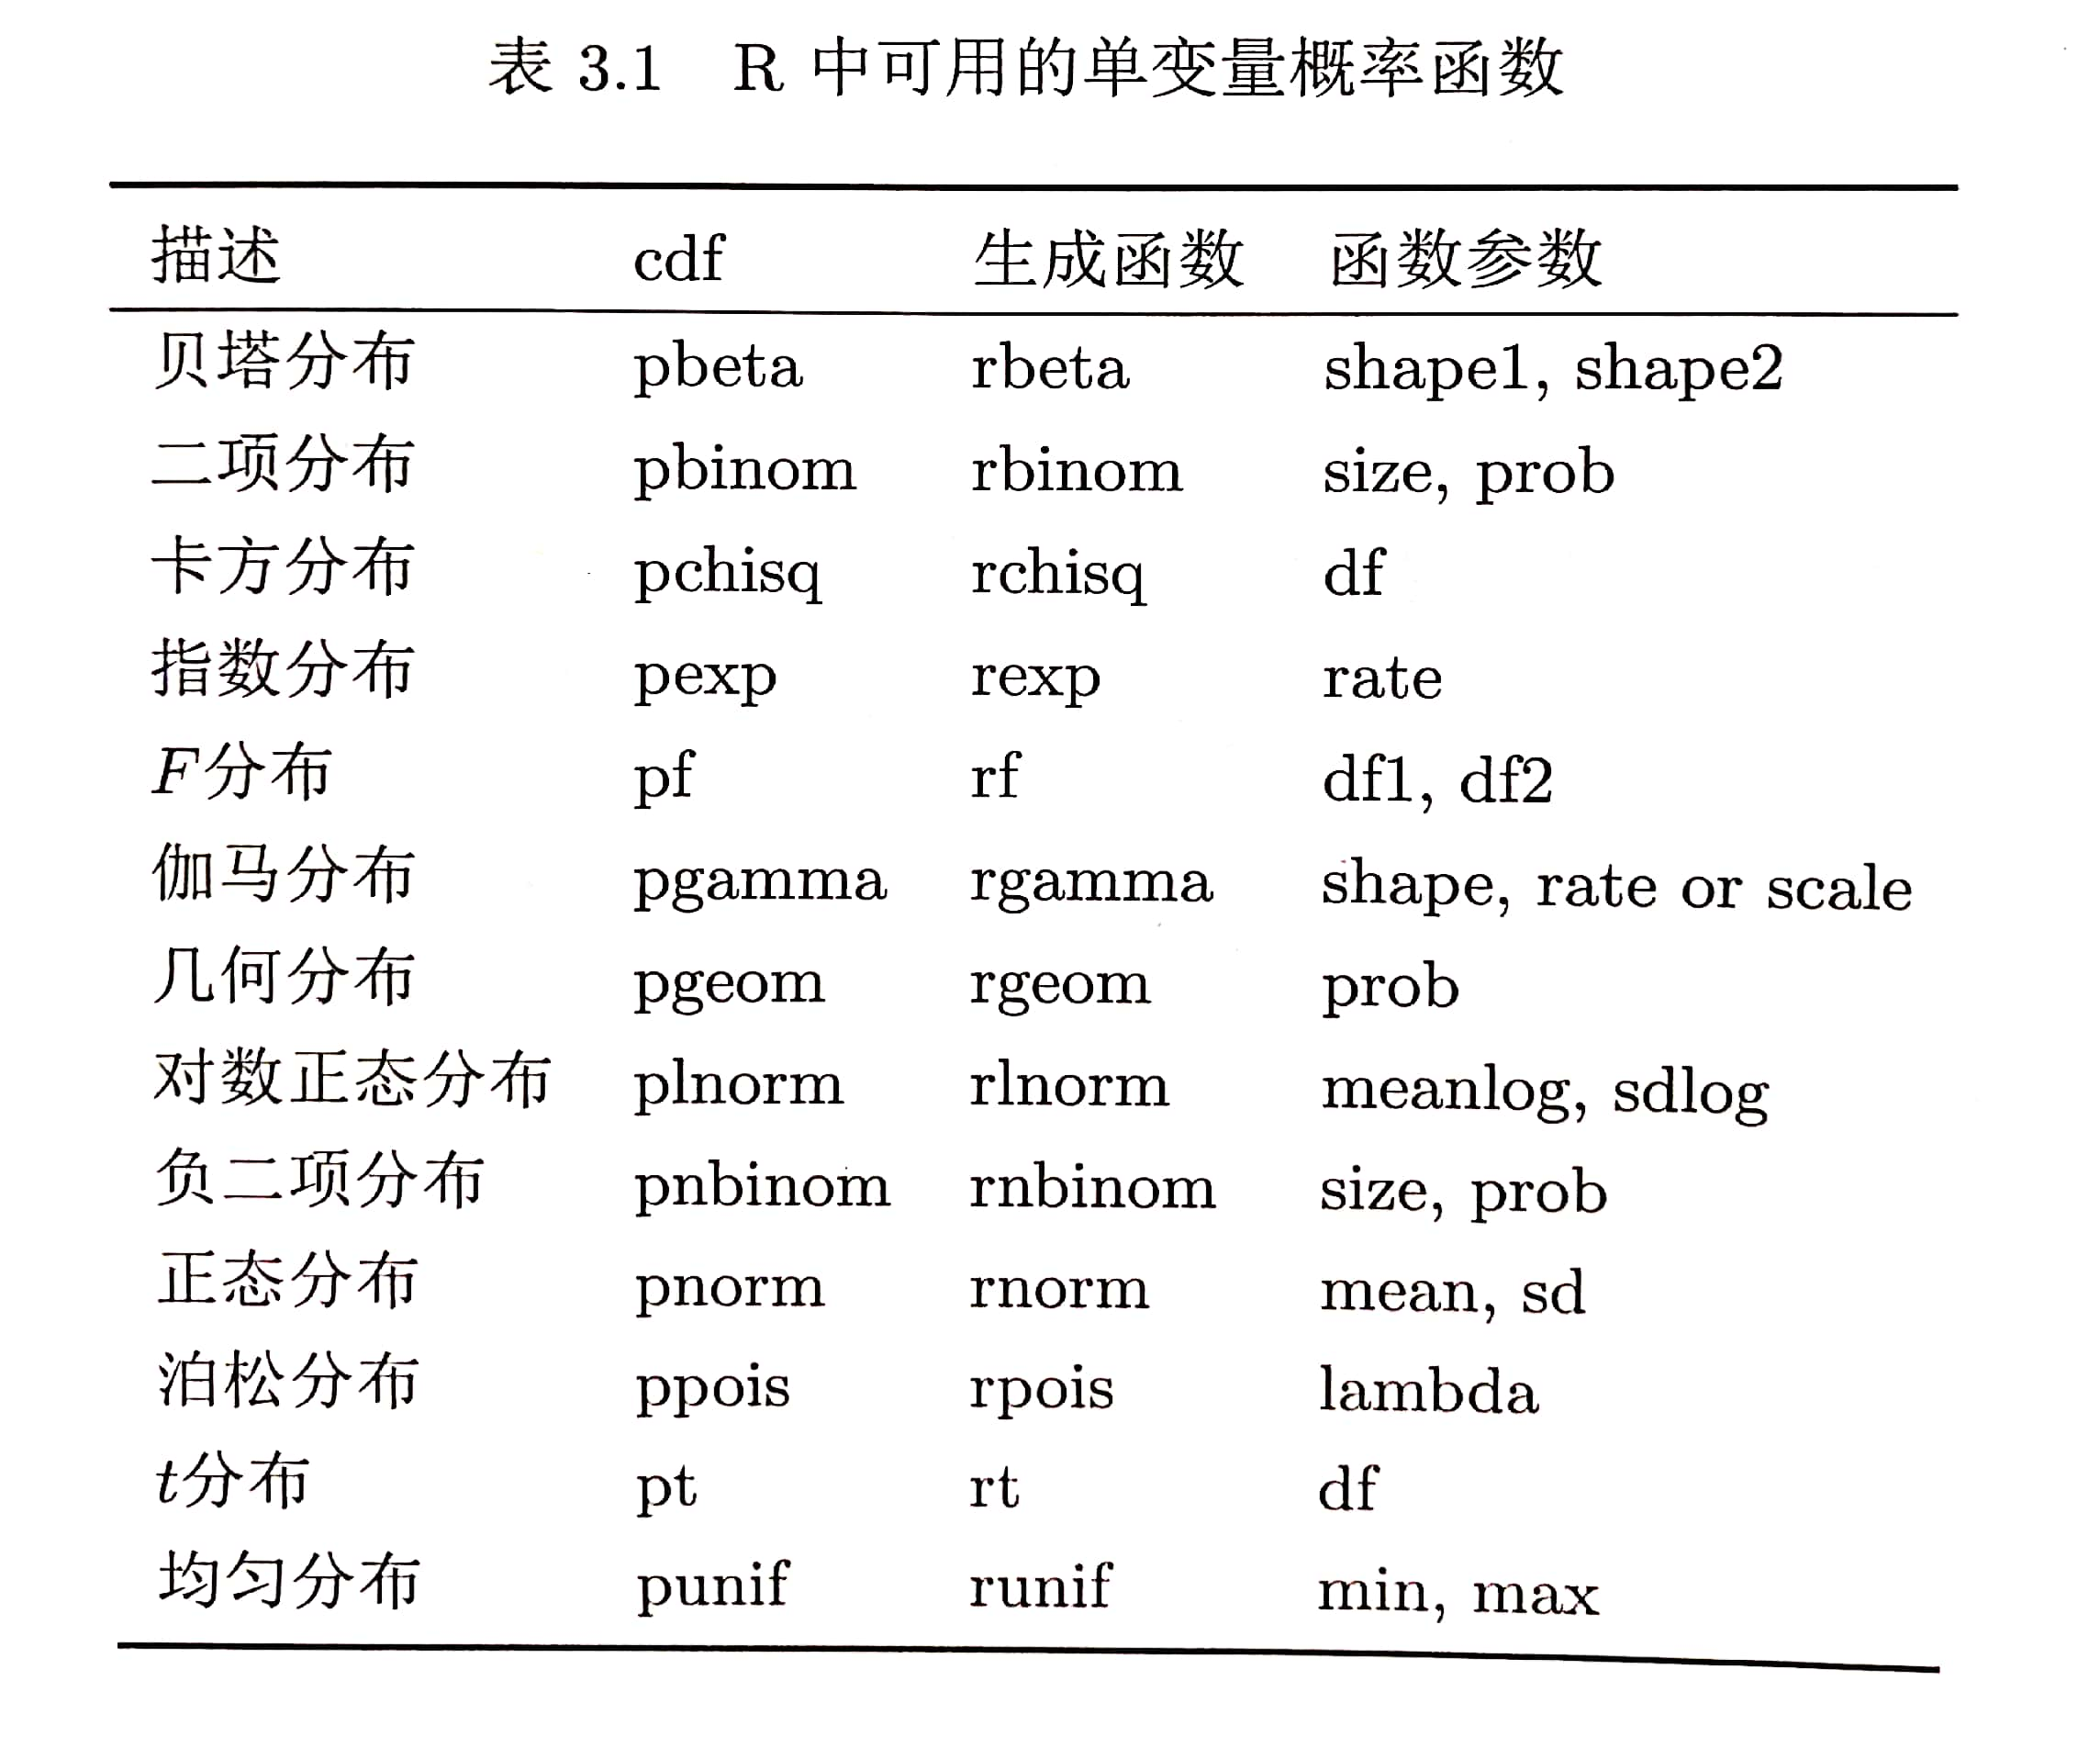
\includegraphics[width=0.7\textwidth]{1.jpg}
\end{figure}

\begin{tcolorbox}[colback=pink!10!white,colframe=pink!100!black]
	\textbf{The Binomial Distribution}
	
	dbinom(x, size, prob, log = FALSE)\\        %pdf或pmf
	pbinom(q, size, prob, lower.tail = TRUE, log.p = FALSE)\\  %cdf
	qbinom(p, size, prob, lower.tail = TRUE, log.p = FALSE)\\  %分位数函数
	rbinom(n, size, prob)     %随机分布生成程序
\end{tcolorbox}
\section{生成随机变量的逆变换法}
原理是万物生一和一生万物,见概率论笔记.

方法概括:
\begin{enumerate}
	\item 推导反函数$F_X^{-1}(u)$.
	\item 编写命令或函数计算$F_X^{-1}(u)$.
	\item 对每个随机变量要求:a) u$\sim$U(0.1); b)令x=$F_X^{-1}(u)$.
\end{enumerate}

\subsection{连续情形下的逆变换法}
\begin{example} 用逆变换法模拟一个pdf:$f_X(x)=3x^2(0<x<1)$的随机样本
\end{example}
令$F_X(x)=x^3,0<x<1, F_X^{-1}(u)=u^{1/3}$,把n个所求的均匀随机数看成一个向量u,这样$u^{1/3}$就成了长度为n的向量且包含样本$x_1,...,x_n$.

\begin{lstlisting}[language=r]
> n<-1000
> u<-runif(n)
> x<-u^(1/3)
> hist(x,prob=TRUE,main=bquote(f(X)==3*x^2))
> y<-seq(0,1,.01)
> lines(y,3*y^2)
\end{lstlisting}
\begin{figure}[H]
	\centering
	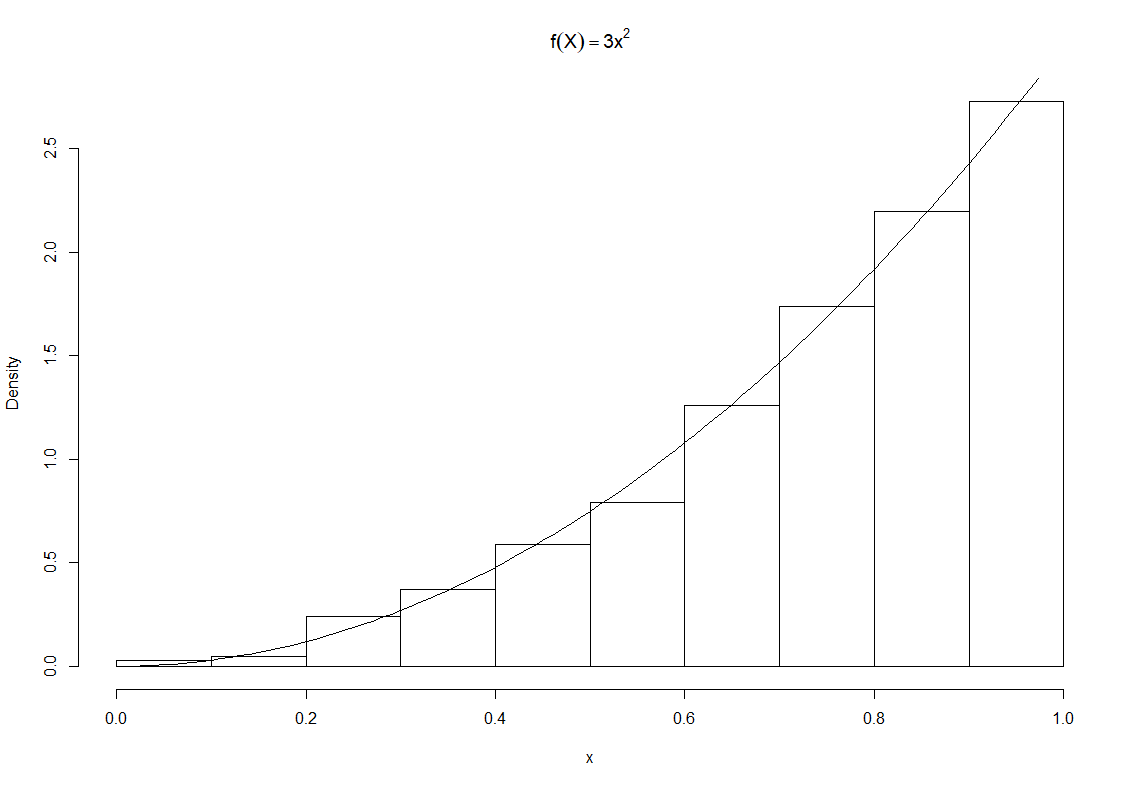
\includegraphics[width=0.7\textwidth]{2.png}
\end{figure}
上图为使用逆变换法得到的随机样本的概率直方图,其中叠加了理论密度函数,显然经验分布和理论分布基本吻合.
\begin{tcolorbox}[colback=blue!7!white,colframe=blue!40]
\textbf{hist函数}用于绘制直方图,下面介绍每个参数的作用;

1)x: 用于绘制直方图的数据,该参数的值为一个向量\\
2) break : 该参数的指定格式有很多种

第一种: 指定一个向量,给出不同的断点. 代码示例:
\begin{lstlisting}[language=r]
data <- c(rep(1, 10), rep(2, 5), rep(3, 6))
hist(data, breaks = c(0.5, 1.5, 2.5, 3.5))	
\end{lstlisting}

第二种:指定分隔好的区间的个数,会根据区间个数自动去计算区间的大小

3)freq: 逻辑值,默认值为TRUE , y轴显示的是每个区间内的频数,FALSE, 代表显示的是频率(= 频数/ 总数)

4)probability : 逻辑值,和 freq 参数的作用正好相反,TRUE 代表频率, FALSE 代表频数

5) labels: 显示在每个柱子上方的标签,

6) axes : 逻辑值,是否显示轴线

7) col : 柱子的填充色

8) border : 柱子的边框的颜色,默认为black, 当border = NA 时, 代表没有边框
\end{tcolorbox}


\begin{tcolorbox}[colback=pink!10!white,colframe=pink!100!black]
标题有数学表达式,可调用expression函数:hist(x,prob=TRUE,main=expression(f(x)==3*x\^2))\\
或者通过main=bquote(f(X)==3*x\^2)得到.
\end{tcolorbox}
\begin{example}
指数分布:用逆变换方法来生成一个服从均值为$1/\lambda$的指数分布的随机样本.
\end{example}
$F_X(x)=1-e^{-\lambda x}$, $F_X^{-1}(u)=-\frac{1}{\lambda}\log (1-u)$.注意到u和1-u具有相同的分布,令$x=-\frac{1}{\lambda}\log (u)$
\begin{lstlisting}[language=r]
> u<-runif(1000)
> lambda<-3
> x<--log(u)/lambda
> hist(x,prob=TRUE)
> y<-seq(0,2.5,.01)
> lines(y,3*exp(-3*y))
\end{lstlisting}
\begin{figure}[H]
	\centering
	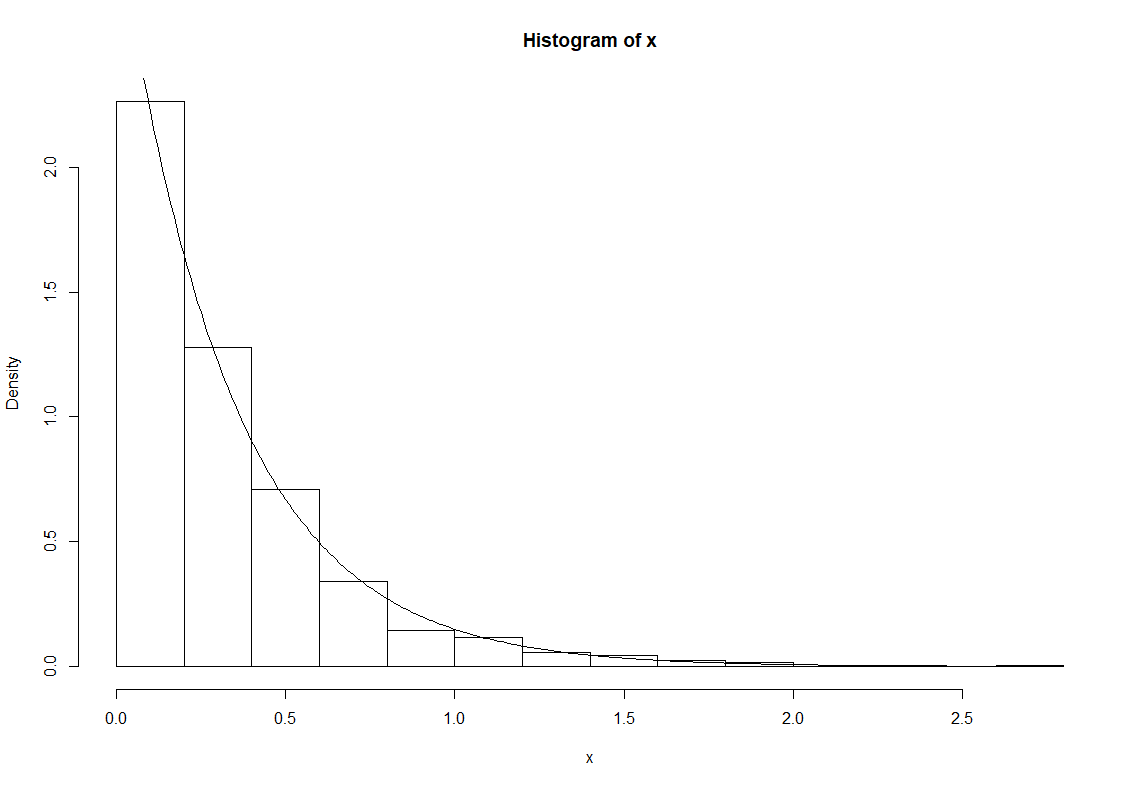
\includegraphics[width=0.5\textwidth]{3.png}
\end{figure}

\begin{tcolorbox}[colback=pink!10!white,colframe=pink!100!black]
rexp(n,m),n表示生成的指数分布随机数的数量,m表示指数分布随机数的均值的倒数,即m=1/mean,默认为1,即默认生成均值为1/m的随机数。
\end{tcolorbox}

\subsection{离散情形下的逆变换法}
如果X是一个离散随机变量并且...<$x_{i-1}<x_i<x_{i+1}$<...是$F_X(x)$的不连续点,那么令$F_X^{-1}(u)=x$,其中$F_X(x_{i-1})$<u$\leq F_X(x_{i})$.

对每个随机变量要求:\\
1. u$ \sim $U(0,1)\\
2.由$F_X(x_{i-1})$<u$\leq F_X(x_{i})$解出$ x_i $

\begin{example}
两点分布:用逆变换方法生成一个伯努利b变量变量构成的随机样本(参数p=0.4).
\end{example}
在R中可能还有更为简单的办法来生成两点分布,而本例则是在最简单的情况下展示了如何计算离散随机变量的逆累积分布函数.

$ F_X(0)=f_X(0)=1-p,F_X(1)=1. $这样,u>0.6, $ F_X^{-1}(u)=1,$当u<0.6, $ F_X^{-1}(u)=0.$
\begin{lstlisting}[language=r]
> n<-1000
> p<-0.4
> u<-runif(n)
> x<-as.integer(u>0.6)
> mean(x)
[1] 0.398
> var(x)
[1] 0.2398358
\end{lstlisting}
比较样本统计量和理论矩,生成样本的均值应接近p=0.4,而样本方差应接近p(1-p)=0.24.
\begin{tcolorbox}[colback=pink!10!white,colframe=pink!100!black]
在R中可以用参数size=1的rbinom函数来生成伯努利样本,也可以对概率分布为(1-p,p)的向量(0,1)取样得到.
\begin{lstlisting}[language=r]
> rbinom(n,size = 1,prob = p)
[1] 0 1 1 0 1 1 0 1 0 1 0 0 0 0 0 0 0 0 0 0 0 0 1 1 1 0 1 0 0 0 1 1 1
[34] 0 1 0 0 0 0 1 0 1 0 0 1 0 1 0 1 0 1 1 0 1 0 0 0 0 0 0 0 1 1 0 0 
[67] 1 0 0 1 1 0 0 0 1 1 1 0 0 0 0 0 0 0 0 1 0 1 1 1 1 0 0 0 1 ......

> sample(c(0,1),size=n,replace=TRUE,prob = c(0.6,0.4))
[1] 0 0 0 0 0 1 1 0 1 0 0 1 1 1 0 0 0 1 0 0 0 0 0 0 1 0 1 0 1 0 1 1 0
[34] 0 0 0 0 1 0 0 0 0 0 1 0 0 0 1 1 0 0 1 0 0 1 0 0 0 1 1 0 0 ......
\end{lstlisting}
你的size是试验次数,n是所需满足该分布的随机数的个数,比如你要生成100个服从B(10,0.5)分布的随机数,命令就应该是 rbinom(100,10,0.5).\\

x是数字的向量。p是概率向量。n是观察的数量。size是试验的数量。prob是每个试验成功的概率。
\end{tcolorbox}

\begin{example}
几何分布:用逆变换法生成一个参数为p=1/4的随机几何样本.
\end{example}
pmf:$ f(x)=pq^x $,其中x=0,1,2,....  F(x)=$ 1-q^{x+1} $.
\begin{tcolorbox}[colback=pink!10!white,colframe=pink!100!black]
这里的F(x)是pmf的等比数列求和.
\end{tcolorbox}
对于每个样本元素,我们需要生成一个服从随即均匀分布的u并解不等式
$$ 1-q^x<u\leq1-q^{1+x} $$
即$$x<\log(1-u)/\log(q)\leq x+1$$
解为$x+1=[\log(1-u)/\log(q)]$, [t]表示取整.
\begin{lstlisting}[language=r]
> n<-1000
> u<-runif(n)
> p<-0.25
> k<-ceiling(log(1-u)/log(1-p))-1
> hist(k)
\end{lstlisting}
\begin{figure}[H]
	\centering
	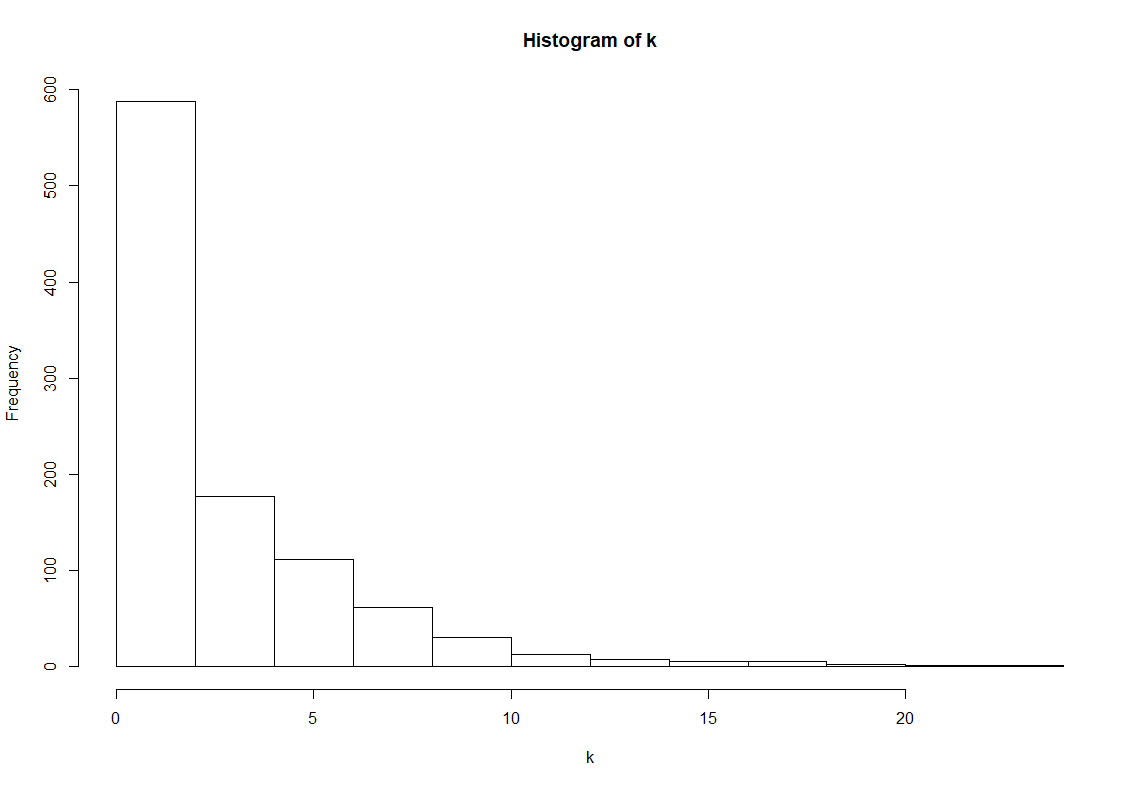
\includegraphics[width=0.6\textwidth]{4.png}
\end{figure}

同样的方法用到泊松分布就会复杂得多,因为我们并没有满足不等式$ F(x-1)<x\leq F(x) $的x的显示表达.

R中rpois函数可以生成随机泊松样本.

\section{接受拒绝法}
设X和Y为随机变量,分别具有pdf或者pmf:f或g,并存在常数c使得
\begin{equation}
	\frac{f(t)}{g(t)}\leq c
\end{equation}
对所有满足$ f(t)>0 $的t都成立.这样接受拒绝法(或称拒绝法)可以用来生成随机变量X.\\
\\
\textbf{接受拒绝法}
\begin{enumerate}
	\item 找到一个随机变量Y,使得其pdf:g满足条件:当$ f(t)>0 $时,$ \frac{f(t)}{g(t)}\leq c $,这就提供了生成随机变量Y的方法.
	\item 对每个要求的随机变量:\\
	1)生成一个随机变量y,使得服从pdf:g的分布;\\
	2)生成一个随机变量u,使得服从U(0,1);\\
	3)如果$ u<\frac{f(y)}{cg(y)} $,则令x=y;否则的话拒绝y,返回步骤1).
\end{enumerate}

在步骤3)中注意,
\begin{equation}
\mathbb{P}(\mbox{接受}|Y)=\mathbb{P}(U<\frac{f(Y)}{cg(Y)}|Y)=\frac{f(Y)}{cg(Y)}
\end{equation}
最后一个等式可以通过对u的累积分布函数进行简单计算即可得到.因此,对任何一次重复接受的全概率为
\begin{equation}
\sum_{y}\mathbb{P}(\mbox{接受}|y)\mathbb{P}(Y=y)=\sum_{y}\frac{f(y)}{cg(y)}g(y)=\frac{1}{c}
\end{equation}
直到接受时所重复的次数服从均值为c的几何分布.这样,平均起来X的每个样本值都需要重复c次.为了提高效率,Y应该取得容易模拟而c则应取得较小.

\begin{example}
\textbf{接受拒绝法}:本例通过$ \beta $ 分布来说明接受拒绝法.在这种方法下为了生成1000个服从$ \alpha=2,\beta=2 $的$ \beta $分布的变量,平均来说需要模拟多少个随机数?这主要取决于$ \frac{f(t)}{g(t)} $的上界c,而这又取决于$ g(x) $的选取.
\end{example}

beta(2,2)的pdf:$ f(x)=6x(1-x) ,0<x<1$.令$ g(x) $为U(0,1)分布的密度函数.这样对于0<x<1都有$ \frac{f(tx}{g(x)}\leq 6 $.因此取c=6.如果满足下面条件,一个服从$ g(x) $分布的随机数x就是被接受的
\begin{equation}
\frac{f(x)}{cg(x)}=\frac{6x(1-x)}{6(1)}=x(1-x)>u
\end{equation}
平均来说,生成一个大小为1000的样本,需要进行cn=6000次重复(12000个随机数).在下面的模拟过程中,重复次数的计数器j不是必须的,添进来知识为了记录生成1000个beta变量实际上需要重复多少次.
\begin{lstlisting}[language=r]
> n<- 1000
> k<- 0 #counter for accepted
> j<- 0 #iterations
> y<- numeric(n)
> while (k<n) {
	+     u<-runif(1)
	+     j<-j+1
	+     x<-runif(1)
	+     if(x*(1-x)>u){
		+         #we accept x
		+         k<-k+1
		+         y[k]<-x
		+     }
	+     
	+ }
> j
[1] 5718
\end{lstlisting}
在这次模拟中,为了生成1000个beta变量总共进行了5718次重复,接下来比较一下经验百分数和理论百分数:
\begin{lstlisting}[language=r]
> p<-seq(.1,.9,.1)
> Qhat<-quantile(y,p)  #经验百分位数
> Q<-qbeta(p,2,2)      #理论百分位数
> se<-sqrt(p*(1-p)/(n*dbeta(Q,2,2)^2))       #q样本分位数的标准差
> round(rbind(Qhat,Q,se),3)
       10%   20%   30%   40%   50%   60%   70%   80%   90%
Qhat 0.180 0.287 0.365 0.431 0.497 0.556 0.617 0.694 0.800
Q    0.196 0.287 0.363 0.433 0.500 0.567 0.637 0.713 0.804
se   0.010 0.010 0.010 0.011 0.011 0.011 0.010 0.010 0.010
\end{lstlisting}
\begin{tcolorbox}[colback=pink!10!white,colframe=pink!100!black]
\begin{enumerate}
	\item \textbf{seq()函数用法}
	
	Sequence Generation: 生成规律的序列。seq是一个带有默认方法的标准通用。\\
	seq(from=1, to=1, by=((to-from)/(length.out-1)),length.out=NULL, along.with=NULL, ...)\\
	seq.int(from, to, by, length.out, along.with, ...)\\
	\\
	by:序列的增量,默认步长为1(可修改)。\\
	length.out:这个序列的输出长度。
\begin{lstlisting}[language=r]
> seq(1, 10, length.out = 6)   # "length.out"= "len"
[1]  1.0  2.8  4.6  6.4  8.2 10.0
\end{lstlisting}
	\item 取百分位比用\textbf{quantile()函数}
\begin{lstlisting}[language=r]
> data <- c(1,2,3,4,5,6,7,8,9,10)
> quantile(data,c(0.25,0.75))
25%  75% 
3.25 7.75 
> quantile(data,seq(0.1,1,0.1))
10%  20%  30%  40%  50%  60%  70%  80%  90% 100% 
1.9  2.8  3.7  4.6  5.5  6.4  7.3  8.2  9.1 10.0 
> unname(quantile(data,seq(0.1,1,0.1)))
[1]  1.9  2.8  3.7  4.6  5.5  6.4  7.3  8.2  9.1 10.0
\end{lstlisting}
\end{enumerate}
\end{tcolorbox}

\begin{tcolorbox}[colback=pink!10!white,colframe=pink!100!black]
\begin{enumerate}
	\item[3.]\textbf{rbind()}
	
	rbind/cbind对数据合并的要求比较严格:合并的变量名必须一致;数据等长
	
	cbind是根据列进行合并,合并的前提是所有数据行数相等。
	
	rbind是根据行进行合并,就是自动往下面顺延,但要求所有数据列数是相同的才能用rbind.

	\item[4.] \textbf{round}是R里的'四舍五入'函数,具体的规则采用banker's rounding,即四舍六入五留双规则(wiki)。
	
	round的原型是round(x, digits = 0), digits设定小数点位置,默认为零即小数点后零位(取整)。
\end{enumerate}
\end{tcolorbox}

\begin{tcolorbox}[colback=blue!7!white,colframe=blue!40]
\textbf{q样本分位数的方差}:

\begin{equation}
Var(\hat{x}_q)=\frac{q(1-q)}{nf(x_q)^2}
\end{equation}
其中f为抽样分布的密度函数.
\end{tcolorbox}

\section{求和变换与混合}
\subsection{卷积}
\textbf{卷积}: $ X_1,...,X_n$ 是相互独立的随机变量,且$ X_j\sim X $.令$ S=X_1+...+X_n $,那么S的分布函数称为X的n重卷积,记为$ F_X^{*(n)} $.

\begin{example}
(卡方分布)本例通过v个正态随机变量二次方的卷积来生成$ \chi^2(v) $随机变量.
\end{example}
如果$ Z_1,...,Z_n $ i.i.d.$ \sim N(0,1)$,那么$ V=Z_1^2+...+Z_n^2 $服从$ \chi^2(v) $分布.生成大小为n的服从$ \chi^2(v) $分布的随机样本:
\begin{enumerate}
	\item 用nv个随机标准正态变量生成一个n$ \times $v的矩阵;
	\item 把上一步的矩阵每个元素二次方;
	\item 计算正态变量二次方行和,每一个行和都是一个来自$ \chi^2(v) $分布的随机观测值.
	\item 导出行和构成的向量
\end{enumerate}

下面给出一个n=1000,v=2的例子:
\begin{lstlisting}[language=r]
> n<-1000
> nu<-2
> X<-matrix(rnorm(n*nu),n,nu)^2
> View(X)
> y<-rowSums(X)
> y<-apply(X,MARGIN = 1,FUN = sum)
> mean(y)
[1] 2.094899
> mean(y^2)
[1] 8.251314
\end{lstlisting}
\begin{tcolorbox}[colback=pink!10!white,colframe=pink!100!black]
函数apply()可以把一个函数应用到数组的各个维度,可以将函数FUN = sum应用到行(MARGIN = 1)上去,来得到矩阵X的行和.
\end{tcolorbox}

\subsection{混合分布}
\textbf{混合分布}: $ X_1,...,$ 是随机变量,$ \theta_i>0 $且$ \sum_i \theta_i=1 $,如果X的分布是一个加权和$ F_X(x)=\sum_i \theta_iF_{X_i}(x) $的形式,则称随机变量X是一个离散的混合变量.

下面比较以下正态随机变量的卷积模拟和混合分布模拟.假设$ X_1\sim N(0,1) $, $ X_2\sim N(3,1) $, 并且它们是互相独立的.表达式$ S=X_1+X_2 $表示卷积,S的分布是均值为3,方差为2的正态分布.

模拟卷积的步骤:
\begin{enumerate}
	\item 生成一个来自N(0,1)的$ x_1 $;
	\item 生成一个来自N(3,1)的$ x_2 $;
	\item 令s=$ x_1+x_2 $
\end{enumerate}

模拟卷积的步骤:
\begin{enumerate}
	\item 生成一个整数k$ \in\left\lbrace 1,2\right\rbrace  $,其中$ \mathbb{P}(1)=\mathbb{P}(2)=0.5 $;
	\item 如果k=1,生成一个来自N(0,1)的x;如果k=2,生成一个来自N(3,1)的x
	\item 令s=$ x_1+x_2 $
\end{enumerate}

\begin{lstlisting}[language=r]
> n<-1000
> x1<-rnorm(n,0,1)
> x2<-rnorm(n,3,1)
> s=x1+x2
> u<-runif(n)
> k<-as.integer(u>0.5)
> x<-k*x1+(1-k)*x2
> 
> par(mfcol=c(1,2))
> hist(s,probability = TRUE)
> hist(x,probability = TRUE)
> par(mfcol=c(1,1))
\end{lstlisting}
\begin{figure}[H]
	\centering
	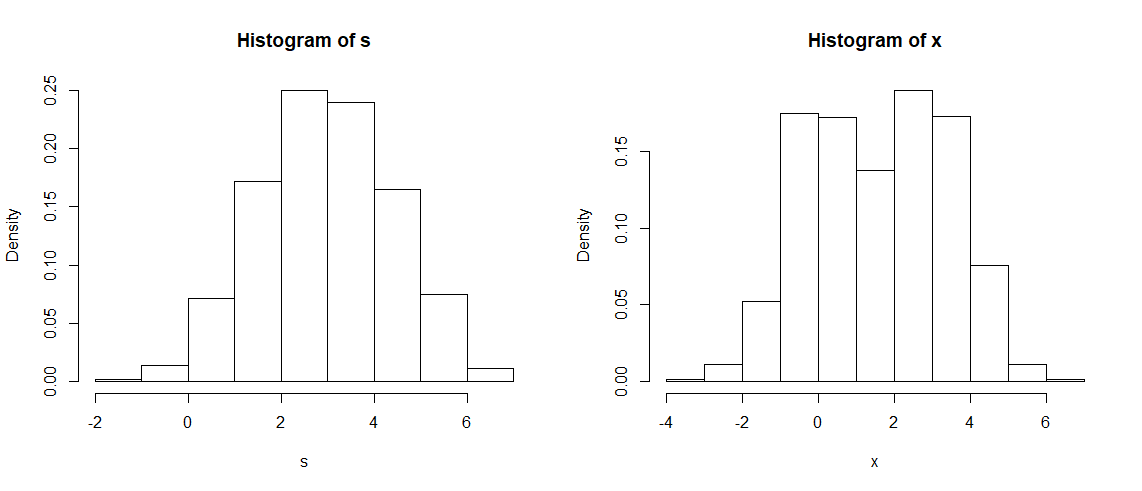
\includegraphics[width=\textwidth]{8.png}
\end{figure}
\begin{tcolorbox}[colback=pink!10!white,colframe=pink!100!black]
par(mfrow=c(1,2))实现一页多图的功能,
其中,通过设定函数par()的各个参数来调整我们的图形\\
mfrow=c(2,2) 就是画4幅图,\\
mfrow=c(3,5),是画15幅图,\\
例如 par(mfrow=c(2,3)) 一个图版显示2行,3列\\
\end{tcolorbox}

\begin{example}
(多个伽马分布的混合变量)
\end{example}
假设$ X_j\sim Gamma(r=3,\lambda_j=1/j) $并且相互独立,混合概率为$ \theta_j=j/15 $, j=1,..,5.混合分布函数:$$F_X(x)=\sum_j^5 \theta_jF_{X_j}(x) $$

生成整数k设定概率在生成随机伽马变量,要用到for循环,在R中不提倡.我们转换称一种向量化方法:
\begin{enumerate}
	\item 生成一个由整数组成的样本$ k_1,...,k_n $,其中$ \mathbb{P}(k)=\theta_k $, k=1,..,5.
	\item 将长度为n的向量$ \lambda=\lambda_k $赋值给rate
	\item 生成大小为n,形参为r,比率向量为rate的gamma样本.
\end{enumerate}

\begin{lstlisting}[language=r]
> n<-5000
> k<-sample(1:5,size=n,replace=TRUE,prob = (1:5)/15)
> rate<-1/k
> x<-rgamma(n,shape = 3,rate = rate)
> plot(density(x),xlim=c(0,40),ylim=c(0,.3),lwd=3,xlab="x",main = "")
> for (i in 1:5) {lines(density(rgamma(n,3,1/i)))}
\end{lstlisting}
\begin{figure}[H]
	\centering
	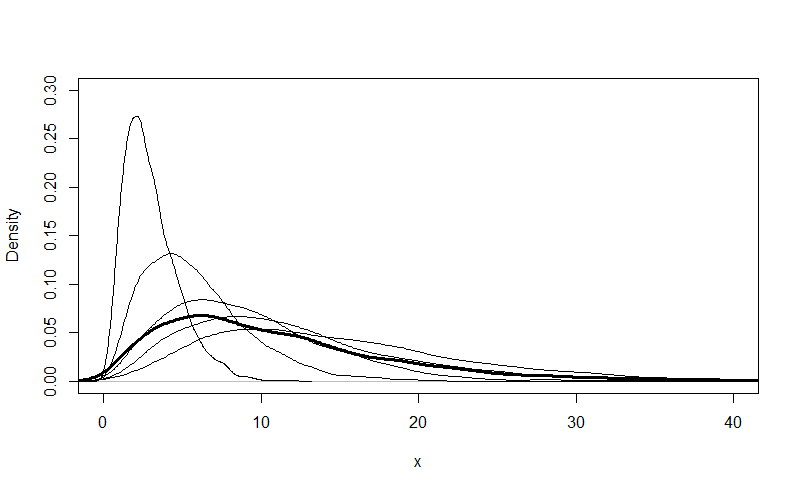
\includegraphics[width=0.8\textwidth]{9.png}
	\caption{多个伽马混合的密度估计图}
\end{figure}

\section{多元分布}
\subsection{多元正态分布}
假设$ \textbf{Z}=Z_{ij} $是一个$ n\times d $矩阵,其中$ Z_{ij} $相互独立服从N(0,1)分布,那么$ \textbf{Z}$的每一行都是一个服从d维标准多元正态分布的随机观测值.

对数据矩阵应用变换$$X=ZQ+J\mu^T$$
其中$ QQ^T=\Sigma $, J是由1组成的列向量.那么所得矩阵X的每一行都是一个服从d维多元正态分布,具有均值$ \mu $和协方差矩阵$ \Sigma $的随机观测值.

\begin{tcolorbox}[colback=blue!7!white,colframe=blue!40]
\textbf{生成多元正态样本的办法}
\begin{enumerate}
	\item 生成包含nd个随机N(0,1)变量的$ n\times d $矩阵Z
	\item 求出$ \Sigma $的分解$ QQ^T=\Sigma $
	\item 应用变换$X=ZQ+J\mu^T$
	\item 导出$ n\times d $矩阵X
\end{enumerate}
\end{tcolorbox}
\begin{tcolorbox}[colback=pink!10!white,colframe=pink!100!black]
	注意矩阵的乘法符号为\%*\%
\end{tcolorbox}

\begin{lstlisting}[language=r]
Z <- matrix(rnorm(n*d),nrow=n,ncol=d)
X <- Z%*%Q + matrix(mu, n, d, byrow=TRUE)
\end{lstlisting}
\begin{tcolorbox}[colback=pink!10!white,colframe=pink!100!black]
matrix(mu, n, d, byrow=TRUE)是$ J\mu^T$,这样处理省去了一次矩阵相乘的运算.byrow的默认参数为false,设为true才能将均值向量逐行填入矩阵.
\end{tcolorbox}
\begin{lstlisting}[language=r]
	
\end{lstlisting}
\begin{lstlisting}[language=r]
	
\end{lstlisting}
\begin{lstlisting}[language=r]
	
\end{lstlisting}
\begin{lstlisting}[language=r]
	
\end{lstlisting}
\begin{lstlisting}[language=r]
	
\end{lstlisting}

\chapter{组合优化}
假设我们的目的在于求函数$ f(\theta) $关于$ \theta=(\theta_1,...,\theta_p) $的最大值,其中$ \theta\in\Theta $且$ \Theta $中元素的个数为有限正整数N.在统计应用中,似然函数经常都依赖于结构参数,而结构参数是用来藐视统计模型形状的,且它有多种互不关联的选择.如果最好的结构参数是已知的,则其余少数参数就很容易被优化.

\section{难题和NP完备性}
在组合优化这样的问题中,关于p个数的组合或排列有许多种,而其中每一种都对应着可能解空间的一个元素,而最大化则需要在这个很大的空间中进行搜索.

考虑\textbf{旅行商问题(traveling salesman problem, TSP)}.旅行商必须访问p个城市中的每一个,且只访问一次后再回到出发地,并要求其总的旅行距离最短.即要求我们在所有可能的路线中寻找总旅行距离最短者.若两个城市之间的距离不依赖于旅行商的旅行方向,则路线共有(p-1)!/2种可能(因为反方向路线是一样的).

我们来考虑一下解决此类问题的难度:
\subsection{P问题、NP问题、NPC问题、NP-hard问题}

先讨论要得到求解此问题所需的算法需要几步,其中每一步都是简单的运算.当然,运算次数依赖于问题的大小,问题的大小是以此问题需要输入次数来衡量的.对于旅行商问题,其大小取决于排列前后p个城市的位置.

\subsubsection{多项式时间(polynomial time)}
时间复杂度并不是表示一个程序解决问题需要花多少时间,而是当程序所处理的问题规模扩大后,程序需要的时间长度对应增长得有多快。也就是说,对于某一个程序,其处理某一个特定数据的效率不能衡量该程序的好坏,而应该\textbf{看当这个数据的规模变大到数百倍后,程序运行时间是否还是一样,或者也跟着快了数百倍,或者变慢了数万倍。}

不管数据有多大,程序处理所花的时间始终是那么多的,我们就说这个程序很好,具有$ O(1) $的时间复杂度,也称\textbf{常数级复杂度};数据规模变得有多大,花的时间也跟着变得有多长,比如找n个数中的最大值这个程序的时间复杂度就是$ O(n) $,为\textbf{线性级复杂度},而像冒泡排序、插入排序等,数据扩大2倍,时间变慢4倍的,时间复杂度$ O(n^2) $,为\textbf{平方级复杂度}。还有一些穷举类的算法,所需时间长度成几何阶数上涨,这就是$ O(a^n) $的\textbf{指数级复杂度},甚至$ O(n!) $的\textbf{阶乘级复杂度}。

容易看出,前面的几类复杂度被分为两种级别,其中后者的复杂度无论如何都远远大于前者。像$ O(1), O(n), O(n^a),O(\ln n) $等,我们把它叫做\textbf{多项式级复杂度},因为它的规模n出现在底数的位置;另一种如$ O(a^n), O(n!) $等,它是\textbf{非多项式级的复杂度},其复杂度计算机往往不能承受。当我们在解决一个问题时,我们选择的算法通常都需要是多项式级的复杂度,非多项式级的复杂度需要的时间太多,往往会超时,除非是数据规模非常小。

\subsubsection{确定性算法与非确定性算法}
\textbf{确定性算法}:设A是求解问题B的一个解决算法,在算法的整个执行过程中,每一步都能得到一个确定的解,这样的算法就是确定性算法。

\textbf{非确定性算法}:设A是求解问题B的一个解决算法,它将问题分解成两部分,分别为猜测阶段和验证阶段,其中
\begin{enumerate}
	\item 猜测阶段:在这个阶段,对问题的一个特定的输入实例x产生一个任意字符串y,在算法的每一次运行时,y的值可能不同,因此,猜测以一种非确定的形式工作。
	\item 验证阶段:在这个阶段,用一个确定性算法(有限时间内)验证。\\
	1)检查在猜测阶段产生的y是否是合适的形式,如果不是,则算法停下来并得到no;\\
	2)如果y是合适的形式,则验证它是否是问题的解,如果是,则算法停下来并得到yes,否则算法停下来并得到no。它是验证所猜测的解的正确性。
\end{enumerate}

\subsubsection{规约/约化}
问题A可以约化为问题B,称为“问题A可规约为问题B”,可以理解为问题B的解一定就是问题A的解,因此解决A不会难于解决B。由此可知问题B的时间复杂度一定大于等于问题A。

《算法导论》中有一个例子:现在有两个问题:求解一个一元一次方程和求解一个一元二次方程。那么我们说,前者可以规约为后者,意即知道如何解一个一元二次方程那么一定能解出一元一次方程。我们可以写出两个程序分别对应两个问题,那么我们能找到一个“规则”,按照这个规则把解一元一次方程程序的输入数据变一下,用在解一元二次方程的程序上,两个程序总能得到一样的结果。这个规则即是:两个方程的对应项系数不变,一元二次方程的二次项系数为0。

从规约的定义中我们看到,一个问题规约为另一个问题,时间复杂度增加了,问题的应用范围也增大了。通过对某些问题的不断规约,我们能够不断寻找复杂度更高,但应用范围更广的算法来代替复杂度虽然低,但只能用于很小的一类问题的算法。存在这样一个NP问题,所有的NP问题都可以约化成它。换句话说,只要解决了这个问题,那么所有的NP问题都解决了。这种问题的存在难以置信,并且更加不可思议的是,这种问题不只一个,它有很多个,它是一类问题。这一类问题就是传说中的NPC问题,也就是NP-完全问题。

\subsubsection{P类问题、NP类问题、NPC问题、NP难问题}
\begin{itemize}
	\item \textbf{P类问题}:能在多项式时间内可解的问题。
	\item \textbf{NP类问题}:在多项式时间内“可验证”的问题。也就是说,不能判定这个问题到底有没有解,而是猜出一个解来在多项式时间内证明这个解是否正确。即该问题的猜测过程是不确定的,而对其某一个解的验证则能够在多项式时间内完成。P类问题属于NP问题,但NP类问题不一定属于P类问题。
	\item \textbf{NPC问题}:存在这样一个NP问题,所有的NP问题都可以约化成它。换句话说,只要解决了这个问题,那么所有的NP问题都解决了。其定义要满足2个条件:\\
	1)它是一个NP问题;\\
	2)所有NP问题都能规约到它。
	\item \textbf{NP难问题}: NP-Hard问题是这样一种问题,它满足NPC问题定义的第二条但不一定要满足第一条(就是说,NP-Hard问题要比 NPC问题的范围广,NP-Hard问题没有限定属于NP),即所有的NP问题都能约化到它,但是他不一定是一个NP问题。NP-Hard问题同样难以找到多项式的算法,但它不列入我们的研究范围,因为它不一定是NP问题。即使NPC问题发现了多项式级的算法,NP-Hard问题有可能仍然无法得到多项式级的算法。事实上,由于NP-Hard放宽了限定条件,它将有可能比所有的NPC问题的时间复杂度更高从而更难以解决。
\end{itemize}
\begin{figure}[H]
	\centering
	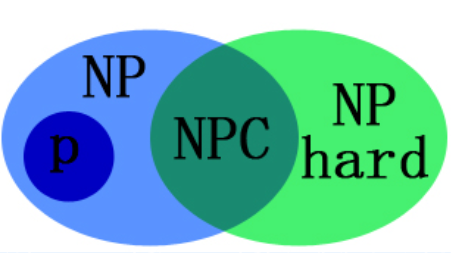
\includegraphics[width=0.3\textwidth]{5.png}
\end{figure}
\subsection{AIC, BIC信息准则}
在多元线性回归问题中,选择合适模型是回归中的基本步骤.对于给定的独立变量Y和候选预测变量$ x_1,...,x_p $,我们需要找到形如$ Y=\beta_0+\sum^{s}_{j=1}\beta_{i_j}x_{i_j}+\epsilon $的最佳模型,其中$ \left\lbrace i_1,...,i_p\right\rbrace  $是$ \left\lbrace 1,...,p\right\rbrace  $的一个子集,$ \epsilon $为随机误差.

很多参数估计问题均采用似然函数作为目标函数,当训练数据足够多时,可以不断提高模型精度,但是以提高模型复杂度为代价的,同时带来一个机器学习中非常普遍的问题——过拟合。所以,模型选择问题在模型复杂度与模型对数据集描述能力(即似然函数)之间寻求最佳平衡。

人们提出许多信息准则,通过加入模型复杂度的惩罚项来避免过拟合问题,此处我们介绍一下常用的两个模型选择方法——\textbf{赤池信息准则(Akaike Information Criterion,AIC)}和\textbf{贝叶斯信息准则(Bayesian Information Criterion,BIC})。
\subsubsection{AIC}
Akaike information criterion.是衡量统计模型拟合优良性(Goodness of fit)的一种标准,由于它为日本统计学家赤池弘次创立和发展的,因此又称赤池信息量准则。它建立在熵的概念基础上,可以权衡所估计模型的复杂度和此模型拟合数据的优良性。
\begin{equation}
AIC=2k-2\ln(L)
\end{equation}
其中k是模型中未知参数个数,L是模型中极大似然函数值似然函数。从一组可供选择的模型中选择最佳模型时,通常选择AIC最小的模型。

当在两个模型之间存在着相当大的差异时,这个差异出现于上式第二项,而当第二项不出现显著性差异时,第一项起作用,从而参数个数少的模型是好的模型。

让n为观察数,RSS(sum square of residue)为残差平方和,那么AIC变为:
\begin{equation}
	AIC=2k+n\ln(RSS/n)
\end{equation}

一般而言,当模型复杂度提高(k增大)时,似然函数L也会增大,从而使AIC变小,但是k过大时,似然函数增速减缓,导致AIC增大,模型过于复杂容易造成过拟合现象。目标是选取AIC最小的模型,AIC不仅要提高模型拟合度(极大似然),而且引入了惩罚项,使模型参数尽可能少,有助于降低过拟合的可能性。可见AIC准则有效且合理地控制了参数的维数k。显然AIC准则追求似然函数尽可能大的同时,k要尽可能的小。

\subsubsection{BIC}
BIC(Bayesian Information Criterion)贝叶斯信息准则与AIC相似,用于模型选择,1978年由Schwarz提出。训练模型时,增加参数数量,也就是增加模型复杂度,会增大似然函数,但是也会导致过拟合现象,针对该问题,AIC和BIC均引入了与模型参数个数相关的惩罚项,BIC的惩罚项比AIC的大,考虑了样本数量,样本数量过多时,可有效防止模型精度过高造成的模型复杂度过高。
\begin{equation}
	BIC=k\ln(n)-2\ln(L)
\end{equation}
其中,k为模型参数个数,n为样本数量,L为似然函数。kln(n)惩罚项在维数过大且训练样本数据相对较少的情况下,可以有效避免出现维度灾难现象。

\subsubsection{AIC与BIC比较}
在模型拟合时,增加参数可使得似然概率增大,但是却引入了额外的变量,因此 AIC 和 BIC 都在目标式中添加了模型参数个数的惩罚项,也就是第二项。当 $ n\geq 8 $ 时,$ k\ln(n)\geq 2k $,所以,BIC 相比 AIC 在大数据量时对模型参数惩罚得更多,导致 BIC 更倾向于选择参数少的简单模型。

\subsection{启发式算法(Heuristic Algorithm)}
对于TSP这样具有挑战性的问题,我们需要对最优化进行新的思考.我们有必要放弃那些能保证找到整体最优(在适当条件下)但在实际可操作的时间内不可能完成的算法.取而代之的是我们转而寻找那些在可容忍的时间内能找到一个好的局部最大值的算法.

有时称这样的算法为\textbf{启发式算法},通俗的解释就是利用类似仿生学的原理,将自然、动物中的一些现象抽象成为算法处理相应问题。当一个问题是NP难问题时,是无法求解到最优解的,因此,用一种相对好的求解算法,去尽可能逼近最优解,得到一个相对优解,在很多实际情况中也是可以接受的.

我们希望利用这些算法平衡速度与整体最优,从而找到一个可与整体最优竞争的候选者(也就是接近最优值).

\textbf{启发式算法的两个基本特征:}\\
1)逐步改进当前的候选解;\\
2)限制任一步迭代仅在局部邻域里寻找.

这两个特征表明启发式算法首先强调的是局部搜索策略.

\subsubsection{启发式算法的定义}
\textbf{启发式算法(Heuristic Algorithm)}有不同的定义:

一种定义为,一个基于直观或经验的构造的算法,对优化问题的实例能给出可接受的计算成本(计算时间、占用空间等)内,给出一个近似最优解,该近似解于真实最优解的偏离程度不一定可以事先预计;

另一种是,启发式算法是一种技术,这种技术使得在可接受的计算成本内去搜寻最好的解,但不一定能保证所得的可行解和最优解,甚至在多数情况下,无法阐述所得解同最优解的近似程度。我比较赞同第二种定义,因为启发式算法现在还没有完备的理论体系,只能视作一种技术。

\textbf{一个容易理解的解释}:

人在解决问题时所采取的一种根据经验规则进行发现的方法。其特点是在解决问题时,利用过去的经验,选择已经行之有效的方法,而不是系统地、以确定的 步骤去寻求答案。启发式解决问题的方法是与算法相对立的。算法是把各种可能性都一一进行尝试,最终能找到问题的答案,但它是在很大的问题空间内,花费大量 的时间和精力才能求得答案。启发式方法则是在有限的搜索空间内,大大减少尝试的数量,能迅速地达到问题的解决。但由于这种方法具有尝试错误的特点,所以也 有失败的可能性。科学家的许多重大发现,常常是利用极为简单的启发式规则。
\begin{tcolorbox}[colback=black!5!white,colframe=black!60!]
文章\textbf{《什么是启发式(heuristic)?》}也许能够增加一点直观印象,尤其它举的例子(用以比较启发式方法和算法)
\\

驾驶汽车到达某人的家,写成算法是这样的:\\
沿167 号高速公路往南行至Puyallup;从South Hill Mall 出口出来后往山上开 4.5 英里; 在一个杂物店旁边的红绿灯路口右转,接着在第一个路口左转;从左边褐色大房子的车道进去,就是North Cedar 路714 号。
\\

用启发式方法来描述则可能是这样:\\
找出上一次我们寄给你的信,照着信上面的寄出地址开车到这个镇;到了之后你问一下我们的房子在哪里。 这里每个人都认识我们——肯定有人会很愿意帮助你的;如果你找不到人,那就找个公共电话亭给我们打电话,我们会出来接你。
\end{tcolorbox}

模拟退火算法(Simulated Annealing Algorithm),人工神经网络(Artificial Neural Network),禁忌搜索(Tabu Search)相继出现。最近,演化算法(Evolutionary Algorithm), 蚁群算法(Ant Algorithms), 拟人拟物算法,量子算法等相继兴起,掀起了研究启发式算法的高潮。由于这些算法简单和有效,而且具有某种智能,因而成为科学计算和人类之间的桥梁。
\begin{figure}[H]
	\centering
	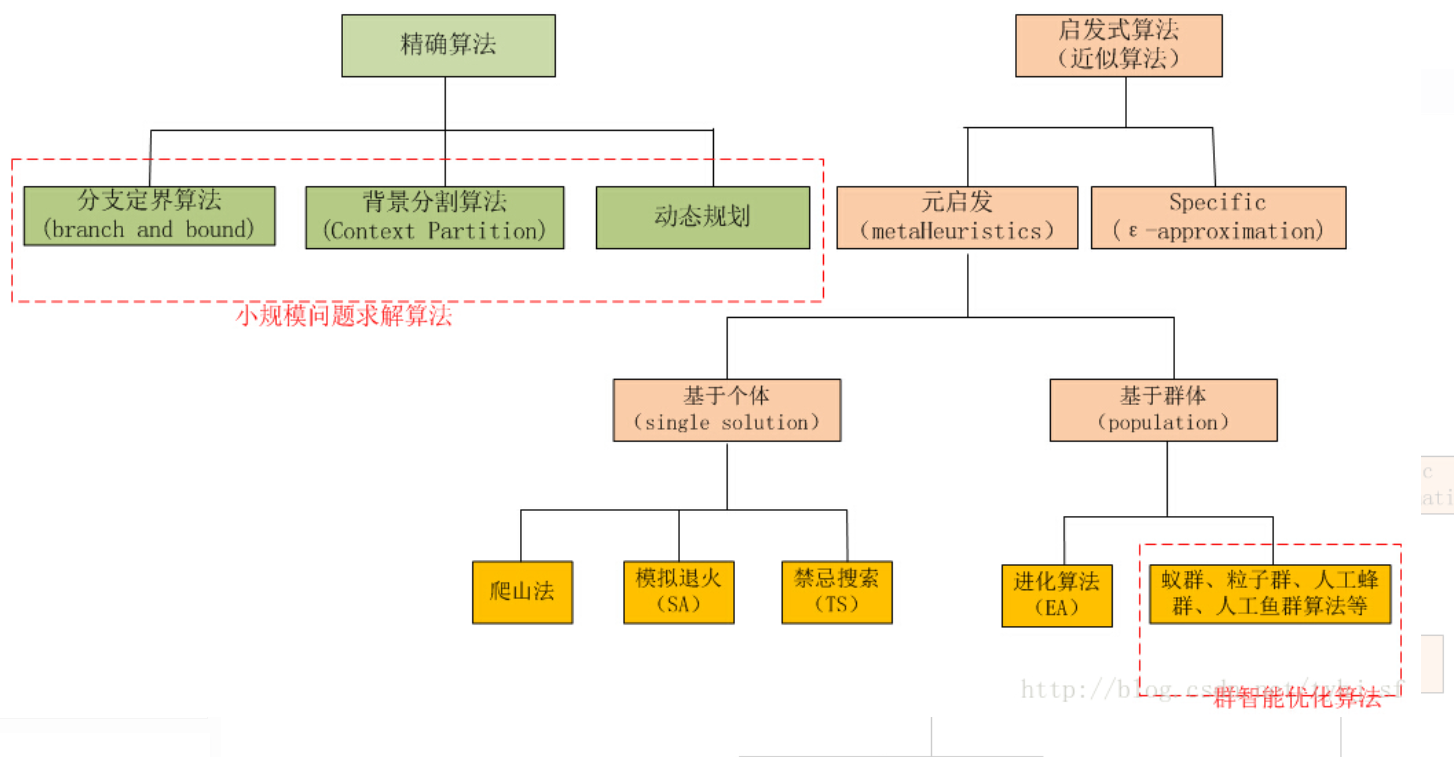
\includegraphics[width=0.9\textwidth]{7.png}
\end{figure}

\section{局部搜索}
在本节将引出某些局部搜索的最简单最一般的变化,如\textbf{k最优}和\textbf{随机初值的局部搜索}.


局部搜索是解决最优化问题的一种启发式算法。对于某些计算起来非常复杂的最优化问题,比如各种NP完全问题,要找到最优解需要的时间随问题规模呈指数增长,因此诞生了各种启发式算法来退而求其次寻找次优解,是一种\textbf{近似算法(Approximate algorithms)},以时间换精度的思想。局部搜索就是其中的一种方法。

基本的局部搜索是一种迭代方法.它用$ \theta^{(t+1)} $来更新当前第t步迭代的候选解$ \theta^{(t)} $.此时的更新称为\textbf{一步移动(move)}.一步或多步可能的移动均来自$ \theta^{(t)} $的一个领域$ N( \theta^{(t)} ) $.

\begin{tcolorbox}[colback=pink!10!white,colframe=pink!100!black]
局部搜索相对于整体或穷尽搜索的\textbf{优点}在于:在每一步迭代,它仅需要在$ \Theta $的很小部分中进行搜索,而$ \Theta $的大部分均不需要验证.

其\textbf{缺点}在于:搜索可能在某个不满意的局部最大值处停止.
\end{tcolorbox}

当前候选解的领域$ N( \theta^{(t)} ) $包含在那些$ \theta^{(t)} $附近的候选解,而这种邻近性通过限制改变当前候选解(用来生成其他候选解的当前解)的次数来保证.\textbf{实际上,我们最好仅对当前候选解进行简单改变,以期得到一个易于搜索与抽样的小邻域.}较复杂的改变是难于概念化和编程的,且运算慢.另外,它们的表现也少有改进,尽管直观上看大邻域产生较差局部最大值的可能性较小.

如果某邻域允许对当前候选解有k种变化,则称此邻域为\textbf{k-邻域},且称对当前候选解的k个特征的改变为\textbf{k-变化}.

有意识地模糊一个邻域地定义就是允许在多种问题中灵活应用这一术语.如在回归模型的选择问题中,一个简单邻域即为由$ \theta^{(t)} $增加或减少一个预测变量的模型集合.

一个局部邻域通常包括几个候选解.在每一步迭代,一个显而易见的策略就是在当前邻域的所有候选解中选择最优的,这就是\textbf{最速上升法(steepest ascent)}.为促进其表现,人们首先会考虑替换随机选取的邻域以使得其目标函数超过它前面的值,这即为\textbf{随机上升法(random ascent)}或\textbf{其次上升法(next ascent)}

如果最速上升法应用\textbf{k-邻域},则称其解为\textbf{k-最优的}.另外,任何由$ \theta^{(t)} $上升到$ \theta^{(t+1)} $的局部搜索算法就是一个上升算法,即使它的上升高度在$ N( \theta^{(t)}) $中可能不是最高的.
	
不管全局最优而只在小邻域中序贯地选择最优值的算法是\textbf{贪婪算法(greedy algorithm)}.一个采用贪婪算法的可能不顾后果而仅考虑当前的最优移动.在从当前候选解邻域选取一个新候选解时,聪明的做法是必须在眼前最佳移动和寻找具有整体竞争力之间保持平衡.为避免一个不好的局部最大值,有时避开$ \theta^{(t)} $方向上的最优邻域可能也是合理的,这一点将在后面看到.


对于k-变化的最速上升法,当k大于1或2时,由于其邻域的大小随k迅速增加,故在当前邻域内的搜索可能非常困难.对于大的k,把k-变化分成几个小的部分,之后把一步k变化分解成几个较小的序列变化,,并结合准许一个或多个较小步作为子集最优(如随机的)的策略.这样的\textbf{可变深度(variable-depth)的局部搜索法}允许一个更好的潜在步偏离当前的候选解,即使它在k-邻域中不可能是最优的.

\subsection{局部搜索--爬山法}
爬山法是向值增加的方向持续移动到简单循环过程,算法在到达一个“峰顶”时终止,此时相邻状态中没有比该“峰顶”更高的值。

爬山法不维护搜索树,当前节点只需要记录当前状态及其目标函数值;爬山法不会前瞻与当前状态不直接相邻的状态的值——“就像健忘的人在大雾中试图登顶珠峰一样”
\begin{tcolorbox}[colback=black!5!white,colframe=black!60!]
function HillClimbing( problem) return 一个局部最优状态\\
    输入: problem\\
局部变量: current, 一个节点\\
          neighbor,一个节点\\
current = MakeNode(Initial-State( problem));\\
loop do\\
   neighbor = a highest-valued successor of  current ;\\
   if VALUE[ neighbor] <= VALUE[ current] then return STATE[ current];\\
   current =  neighbor ;
\end{tcolorbox}

爬山法又称贪婪局部搜索,只是选择相邻状态中最好的一个。尽管贪婪是七宗罪之一,但是贪婪算法往往能够获得很好的效果。当然,爬山法会遇到以下问题:
\begin{enumerate}
	\item 局部极值
	\item 山脊:造成一系列的局部极值
	\item 高原:平坦的局部极值区域——解决办法:继续侧向移动
\end{enumerate}

\begin{figure}[H]
	\centering
	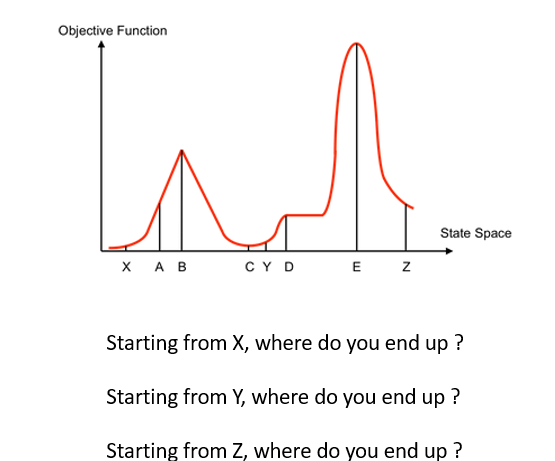
\includegraphics[width=0.7\textwidth]{10.png}
\end{figure}

\subsubsection{爬山法的变体形式}
\begin{enumerate}
	\item \textbf{随机爬山法:}
	在上山移动中,随机选择下一步,选择的概率随着上山移动到陡峭程度而变化;
	\item \textbf{首选爬山法}
	随机地生成后继节点直到生成一个优于当前节点的后继
	\item \textbf{随机重新开始的爬山法}
	“如果一开始没有成功,那么尝试,继续尝试”
	算法通过随机生成的初始状态来进行一系列的爬山法搜索,找到目标时停止搜索。
	
	该算法以概率1接近于完备:因为算法最终会生成一个目标状态作为初始状态
\end{enumerate}


\subsection{随机初值的局部搜索(Random Starts Local Search) }
上升算法经常收敛于一个不具有整体竞争力的局部最大值,\textbf{随机初值的局部搜索(random starts local search)}技术即为克服这一不足的一种方法.此时,从多个初值出发,重复运行一个简单的上升算法直到结束.这些初值都是随机选取的额,选取初值的一个最简单方法即是在$ \Theta $中独立且均匀地随机选取.某些精致方法可能考虑某种类型的分层抽样,而其层是通过某些试运行以期分解$ \Theta $成几个具有不同收敛行为的区域来得到.

仅依赖随机初值来避免局部最大值看来不是令人很满意.在后面几节,我们将引入一些修改的局部搜索法,而这些修改的目的在于每一次运行均有机会求得具有整体竞争力的候选解,可也可能是整体最优值.当然也可结合应用多重随机初值的策略和这些修改方法以提供一个更可信的最优解.

\begin{example}
\textbf{(棒球运动员的薪水)}:实际上,如果时间允许采用多个随机初值,则由于随机初值的局部搜索法易于编程且运行速度快,故它是一种非常有效的方法.这里,我们考虑它在回归模型选择问题上的应用.

我们将薪水变量的对数作为响应变量,其目的在于应用线性回归模型来求取预测薪水对数的最优预测变量子集.数据中有27个变量反映棒球运动员表现,如假设任一模型均有截距项,则搜索空间共有$ 2^{27}=134217728 $个可能的模型.
\end{example}

读入数据baseball.dat:
\begin{lstlisting}[language=r]
> baseball.dat = read.table(file.choose(),header=TRUE)
> View(baseball.dat)
\end{lstlisting}
\begin{tcolorbox}[colback=pink!10!white,colframe=pink!100!black]
\textbf{read.table的语法规则:}
read.table(file,header=FALSE,sep="",...)

用file.choose()选择数据文件。
read.table(file.choose(),header=T)
\end{tcolorbox}
令freeagent(自由队员)和arbitration(仲裁)为因子型,
\begin{lstlisting}[language=r]
> baseball.dat$freeagent = factor(baseball.dat$freeagent)
> baseball.dat$arbitration = factor(baseball.dat$arbitration)
> str(baseball.dat)
'data.frame':	337 obs. of  28 variables:
$ salary      : int  3300 2600 2500 2475 2313 2175 600 460 240 200 ...
$ average     : num  0.272 0.269 0.249 0.26 0.273 0.291 0.258 0.228 ...
$ obp         : num  0.302 0.335 0.337 0.292 0.346 0.379 0.37 0.279 ...
$ runs        : int  69 58 54 59 87 104 34 16 40 39 ...
$ hits        : int  153 111 115 128 169 170 86 38 61 64 ...
$ doubles     : int  21 17 15 22 28 32 14 7 11 10 ...
$ triples     : int  4 2 1 7 5 2 1 2 0 1 ...
$ homeruns    : int  31 18 17 12 8 26 14 3 1 10 ...
$ rbis        : int  104 66 73 50 58 100 38 21 18 33 ...
$ walks       : int  22 39 63 23 70 87 15 11 24 14 ...
$ sos         : int  80 69 116 64 53 89 45 32 26 96 ...
$ sbs         : int  4 0 6 21 3 22 0 2 14 13 ...
$ errors      : int  4 4 6 22 9 5 11 4 3 7 ...
$ freeagent   : Factor w/ 2 levels "0","1": 2 2 2 1 1 2 2 1 1 1 ...
$ arbitration : Factor w/ 2 levels "0","1": 1 1 1 2 2 1 1 1 1 1 ...
$ runsperso   : num  0.863 0.841 0.466 0.922 1.641 ...
$ hitsperso   : num  1.913 1.609 0.991 2 3.189 ...
$ hrsperso    : num  0.388 0.261 0.147 0.188 0.151 ...
$ rbisperso   : num  1.3 0.957 0.629 0.781 1.094 ...
$ walksperso  : num  0.275 0.565 0.543 0.359 1.321 ...
$ obppererror : num  0.0755 0.0838 0.0562 0.0133 0.0384 0.0343 ...
$ runspererror: num  17.25 14.5 9 2.68 9.67 ...
$ hitspererror: num  38.25 27.75 19.17 5.82 18.78 ...
$ hrspererror : num  7.75 4.5 2.833 0.545 0.889 ...
$ soserrors   : int  320 276 696 1408 477 445 495 128 78 672 ...
$ sbsobp      : num  1.21 0 2.02 6.13 1.04 ...
$ sbsruns     : int  276 0 324 1239 261 2288 0 32 560 507 ...
$ sbshits     : int  612 0 690 2688 507 3740 0 76 854 832 ...
\end{lstlisting}

单独提出所有的预测变量,同时给薪水变量作对数处理.
\begin{lstlisting}[language=r]
> baseball.sub = baseball.dat[,-1]
> salary.log = log(baseball.dat$salary)
\end{lstlisting}
\begin{enumerate}
	\item \textbf{n} = number of observations in the data set
	\item \textbf{m} = number of predictors in the data set
	\item \textbf{num.starts} = number of random starts
	\item \textbf{runs} = matrix containing the random starts where each row is a vector of the parameters included for the model (1 = included, 0 = omitted)
	\item \textbf{runs.aic}	= AIC values for the best model found for each of the random starts
	\item \textbf{itr} = number of iterations for each random start
\end{enumerate}

\begin{lstlisting}[language=r]
> n = length(salary.log)
> m = length(baseball.sub[1,])
> num.starts = 5
> itr = 15
> runs.aic = matrix(0,num.starts,itr)
\end{lstlisting}

用随机初值的局部搜索方法来求使AIC最小的相应回归模型的图例.由于可把此问题看成求负AIC的最大值问题,于是可用上升搜索来衡量其表现.邻域仅局限于对当前模型添加或去掉一个变量的一个变化来生成.从5个随机选取的变量子集(即5个初值)开始搜索,且分配给每个初值14步.每步移动均由最速上升所决定.由于每步最速上升均要求搜索27个邻域,于是要求对目标函数进行$ 27\times 14\times 5=1890 $次计算.


\begin{lstlisting}[language=r]
> # INITIALIZES STARTING RUNS
> set.seed(19676) 
> for(i in 1:num.starts){runs[i,] = rbinom(m,1,.5)}
\end{lstlisting}

\begin{lstlisting}[language=r]
> ## MAIN
> for(k in 1:num.starts){
	+ 	run.current = runs[k,]
	+ 
	+ 	# ITERATES EACH RANDOM START
	+ 	for(j in 1:itr){
		+ 	run.vars = baseball.sub[,run.current==1]
		+ 	g = lm(salary.log~.,run.vars)
		+ 	run.aic = extractAIC(g)[2]
		+ 	run.next = run.current
		+ 
		+ 	# TESTS ALL MODELS IN THE 1-NEIGHBORHOOD AND 
		+ 	# SELECTS THE MODEL WITH THE LOWEST AIC
		+ 	for(i in 1:m){
			+ 	run.step = run.current
			+ 	run.step[i] = !run.current[i]
			+ 	run.vars = baseball.sub[,run.step==1]
			+ 	g = lm(salary.log~.,run.vars)
			+ 	run.step.aic = extractAIC(g)[2]
			+ 	if(run.step.aic < run.aic){
				+ 	run.next = run.step
				+ 	run.aic = run.step.aic
				+ 	}
			+ 	}
		+ 	run.current = run.next
		+ 	runs.aic[k,j]=run.aic
		+ 	}
	+ 	runs[k,] = run.current
	+ }
\end{lstlisting}
\begin{lstlisting}[language=r]
> ## OUTPUT
> runs 		# LISTS OF PREDICTORS
     [,1] [,2] [,3] [,4] [,5] [,6] [,7] [,8] [,9] [,10] [,11] [,12]
[1,]    0    0    1    0    0    1    0    1    0     0     0     1
[2,]    0    1    1    0    0    1    0    1    0     1     0     0
[3,]    0    1    1    0    0    1    0    1    0     1     0     0
[4,]    0    0    1    0    0    0    0    1    1     1     0     0
[5,]    0    0    1    0    0    0    0    1    0     1     0     1
     [,13] [,14] [,15] [,16] [,17] [,18] [,19] [,20] [,21] [,22] [,23]
[1,]     1     1     0     0     0     0     0     0     1     1     0
[2,]     1     1     1     1     0     0     0     0     0     0     0
[3,]     1     1     1     1     0     0     0     0     0     0     0
[4,]     1     1     0     0     0     0     1     1     1     1     0
[5,]     1     1     1     1     0     0     0     1     0     1     0
     [,24] [,25] [,26] [,27]
[1,]     1     1     0     0
[2,]     1     1     1     0
[3,]     1     1     1     0
[4,]     0     0     0     0
[5,]     0     1     0     1
> runs.aic 	# AIC VALUES
          [,1]      [,2]      [,3]      [,4]      [,5]      [,6]
[1,] -381.1793 -394.2750 -399.7520 -404.2200 -406.2200 -408.2195
[2,] -399.0655 -401.5732 -407.0510 -409.0429 -410.9505 -412.8614
[3,] -408.4422 -413.0112 -415.0096 -415.6115 -417.5230 -417.7187
[4,] -398.9160 -406.4152 -408.4151 -410.3917 -411.4037 -411.9585
[5,] -403.7879 -405.7847 -407.7694 -409.7152 -411.0934 -413.0607
          [,7]      [,8]      [,9]     [,10]     [,11]     [,12]
[1,] -410.1393 -411.9637 -413.0388 -413.0388 -413.0388 -413.0388
[2,] -414.4943 -416.2275 -417.2010 -418.0125 -418.9472 -418.9472
[3,] -418.9472 -418.9472 -418.9472 -418.9472 -418.9472 -418.9472
[4,] -412.8700 -414.0506 -415.4118 -415.5199 -415.5199 -415.5199
[5,] -414.6612 -416.1504 -416.1504 -416.1504 -416.1504 -416.1504
         [,13]     [,14]     [,15]
[1,] -413.0388 -413.0388 -413.0388
[2,] -418.9472 -418.9472 -418.9472
[3,] -418.9472 -418.9472 -418.9472
[4,] -415.5199 -415.5199 -415.5199
[5,] -416.1504 -416.1504 -416.1504
\end{lstlisting}
\begin{lstlisting}[language=r]
> ##PLOT
> plot(1:(itr*num.starts),-c(t(runs.aic)),xlab="Cumulative Iterations",
+   ylab="Negative AIC",ylim=c(360,420),type="n")
> for(i in 1:num.starts) {
	+   lines((i-1)*itr+(1:itr),-runs.aic[i,]) }
\end{lstlisting}
\begin{figure}[H]
	\centering
	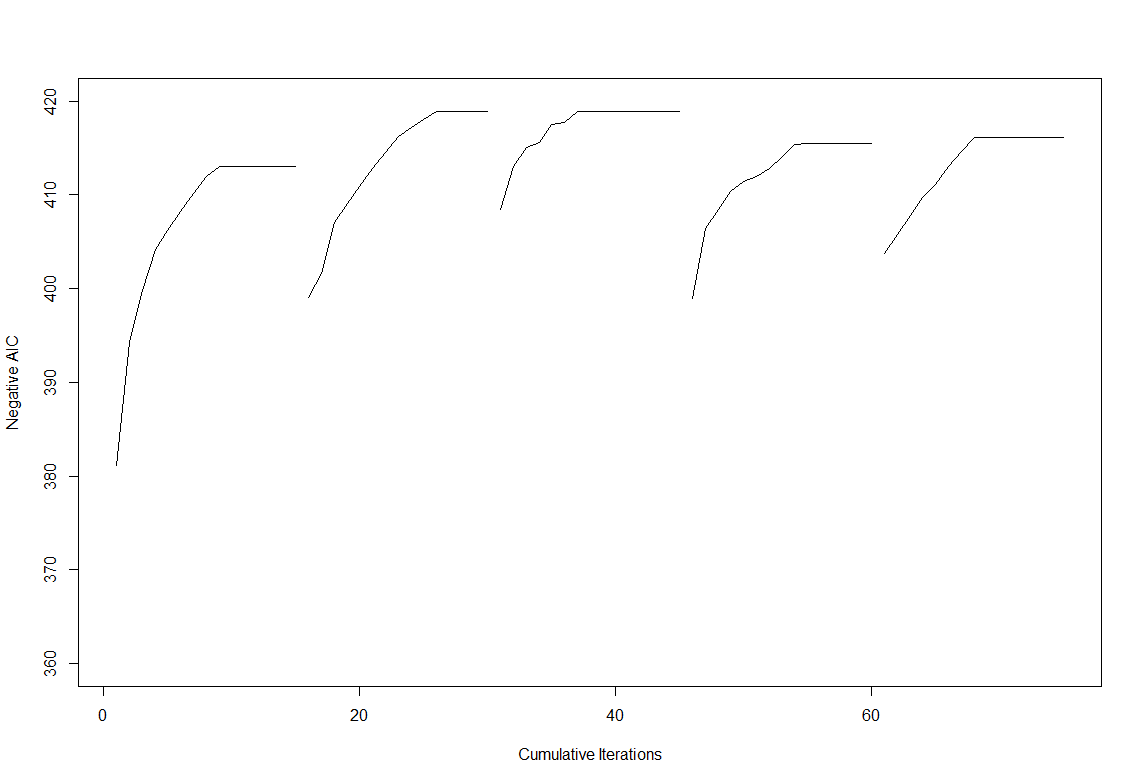
\includegraphics[width=\textwidth]{6.png}
\end{figure}

\section{禁忌搜索算法(Tabu  Search)}
\textbf{先从爬山算法说起}

爬山算法从当前的节点开始,和周围的邻居节点的值进行比较。 如果当前节点是最大的,那么返回当前节点,作为最大值 (既山峰最高点);反之就用最高的邻居节点来,替换当前节点,从而实现向山峰的高处攀爬的目的。如此循环直到达到最高点。因为不是全面搜索,所以结果可能不是最佳。

\textbf{再到局部搜索算法}

局部搜索算法是从爬山法改进而来的。局部搜索算法的基本思想:在搜索过程中,始终选择当前点的邻居中与离目标最近者的方向搜索。同样,局部搜索得到的解不一定是最优解。

\textbf{然后到禁忌搜索算法}

为了找到“全局最优解”,就不应该执着于某一个特定的区域。于是人们对局部搜索进行了改进,得出了禁忌搜索算法。

\textbf{禁忌(Tabu Search)算法}是一种亚启发式(meta-heuristic)随机搜索算法,它从一个初始可行解出发,选择一系列的特定搜索方向(移动)作为试探,选择实现让特定的目标函数值变化最多的移动。为了避免陷入局部最优解,TS搜索中采用了一种灵活的“记忆”技术,对已经进行的优化过程进行记录和选择,指导下一步的搜索方向,这就是Tabu表的建立。

\begin{figure}[H]
	\centering
	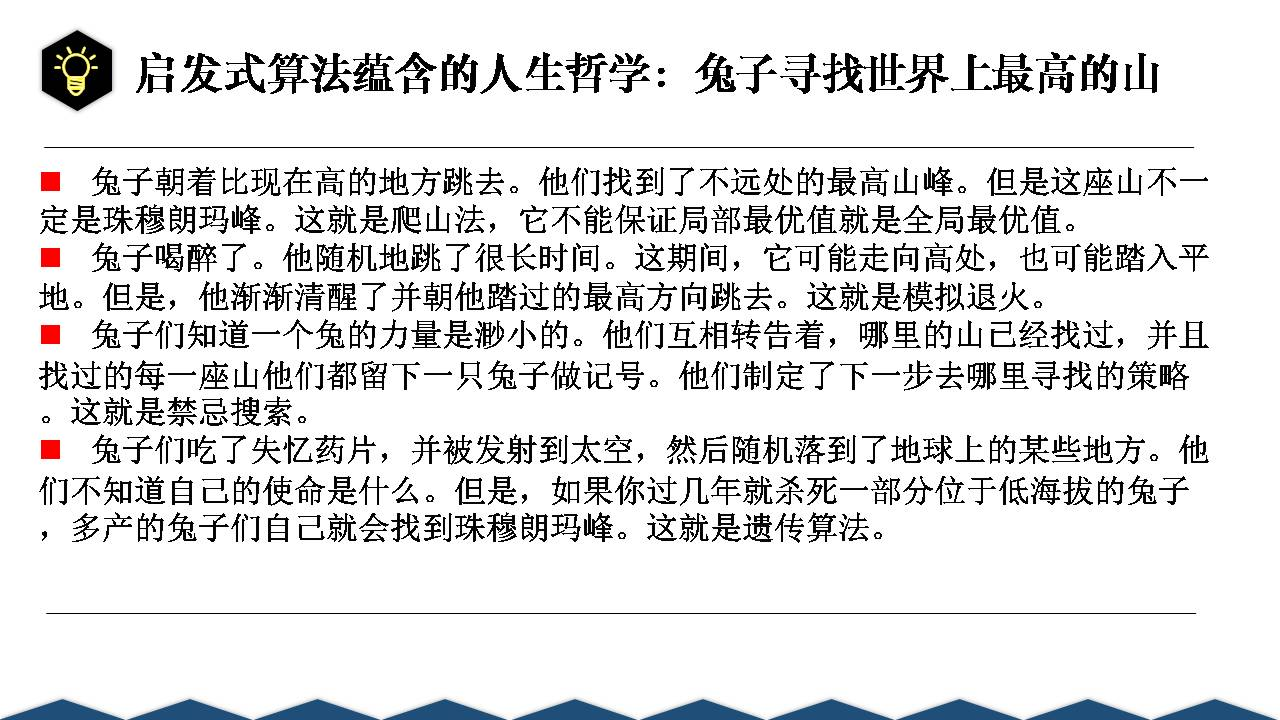
\includegraphics[width=\textwidth]{11.jpg}
\end{figure}

\textbf{禁忌搜索算法}:

兔子寻找世界上最高的山.兔子们找到了泰山,它们之中的一只就会留守在这里,其他的再去别的地方寻找。当兔子们再寻找时,一般地会有意识地避开泰山,因为他们知道,这里已经找过,并且有一只兔子在那里看着了。这就是禁忌搜索中“\textbf{禁忌表(tabu list)}”的含义。

那只留在泰山的兔子一般不会就安家在那里了,它会在一定时间后重新回到找最高峰的大军,因为这个时候已经有了许多新的消息,泰山毕竟也有一个不错的高度,需要重新考虑这个归队时间,在禁忌搜索里面叫做“\textbf{禁忌长度(tabu length)}”;

如果在搜索的过程中,留守泰山的兔子还没有归队,但是找到的地方全是华北平原等比较低的地方,兔子们就不得不再次考虑选中泰山,也就是说,当一个有兔子留守的地方优越性太突出,超过了“best so far"的状态,就可以不顾及有没有兔子留守,都把这个地方考虑进来,这就叫“\textbf{特赦准则(aspiration criterion)}”。这三个概念就这样一大圈后,把找到的几个山峰一比较,珠穆朗玛峰脱颖而出。是禁忌搜索和一般搜索准则最不同的地方,算法的优化也关键在这里。

\subsection{算法概述:主要思路}
1.在搜索中,构造一个短期循环记忆表-禁忌表,禁忌表中存放刚刚进行过的|T|(T称为禁忌表)个邻居的移动,这种移动即解的简单变化。

2.禁忌表中的移动称为禁忌移动。对于进入禁忌表中的移动,在以后的|T|次循环内是禁止的,以避免回到原来的解,从而避免陷入循环。|T|次循环后禁忌解除.

3.禁忌表是一个循环表,在搜索过程中被循环的修改,使禁忌表始终保持|T|个移动.

4.即使引入了禁忌表,禁忌搜索仍可能出现循环。因此,必须给定停止准则以避免出现循环。当迭代内所发现的最好解无法改进或无法离开它时,算法停止。

\subsection{算法原理}

禁忌搜索算法是组合优化算法的一种,是局部搜索算法的扩展。禁忌搜索算法是人工智能在组合优化算法中的一个成功应用。禁忌搜索算法的特点是采用了禁忌技术。所谓禁忌就是禁止重复前面的工作。禁忌搜索算法用一个禁忌表记录下已经到达过的局部最优点,在下一次搜索中,利用禁忌表中的信息不再或有选择地搜索这些点。

禁忌搜索算法涉及侯选集合、禁忌对象、评价函数、特赦规则、记忆频率信息等概念。

\subsubsection{邻域}

一个组合优化问题可用三参数(D,F,f)表示,D表示决策变量的定义域,F表示可行解区域,F中的任何一个元素称为该问题的可行解。f是目标函数,满足$f(x^*)=min\left\lbrace f(x)|x\in F\right\rbrace  $的可行解x*称为该问题的最优解。

\textbf{定义l:}对于组合优化问题(D,F,f),D上的一个映射:
$$ N:S\in D\rightarrow N(S)\in 2^D $$称为D的一个邻域映射,其中$ 2^D $表示D的所有子集构成的集合, N(S)称为S的领域,$ S'\in N(S) $称为S的一个邻居。

\subsubsection{候选集合和评价函数}

\textbf{侯选集合}由邻域中的邻居组成。常规的方法是从邻域中选择若干个目标值或评价值最佳的邻居入选。

\textbf{评价函数}是侯选集合元素选取的一个评价公式,侯选集合的元素通过评价函数值来选取。以目标函数作为评价函数是比较容易理解的。目标值是一个非常直观的指标,但有时为了方便或易于计算,会采用其他函数来取代目标函数。

\subsubsection{禁忌对象和禁忌长度}
当考虑来自$ \theta^{(t)} $的移动时,我们要计算目标函数在$ \theta^{(t)} $的每一个邻域内的增量.通常采用提供的最大增量的邻域作为$ \theta^{(t+1)} $,这即对应着\textbf{最速上升法}.然而,如果在$ \theta^{(t)} $的任意邻域内目标函数均不增加时,则通常选取$ \theta^{(t+1)} $为使减少量最小的邻域,这即为\textbf{适度下降法}.如果仅用这两个准则,则算法很快被捕获且收敛到一个局部最大值.经一步适度下降后,下一步将回到刚离开的山顶,且接下来进行循环.

为了避免遮掩的循环,在算法中引进一个暂时限制移动的\textbf{禁忌表(tabu list)}.禁忌表中的两个主要指标是禁忌对象和禁忌长度。

除去禁忌表后的邻域:
$$ N(\theta^{(t)},H^{(t)})= \left\lbrace \theta: \theta \in N(\theta^{(t)})且没有\theta 的属性当前是被禁止的\right\rbrace $$

禁忌算法中,由于我们要避免一些操作的重复进行,就要将一些元素放到禁忌表中以禁止对这些元素进行操作,这些元素就是我们指的\textbf{禁忌对象}。

\textbf{禁忌长度(禁忌期限)}是被禁对象不允许选取的迭代次数。一般是给被禁对象一个数x一个禁忌长度t,要求对象x在t步迭代内被禁,在禁忌表中采用$ tabu(x)=t $记忆,每迭代一步,该项指标做运算
$ tabu(x)=t-1 $直到$ tabu(x)=0 $时解禁。于是,我们可将所有元素分成两类,被禁元素和自由元素。禁忌长度t的选取可以有多种方法,例如t=常数,或者$ t=[\sqrt{n}] $,其中n为领域中邻居的个数;这种规则容易在算法中实现。

\subsubsection{特赦规则和记忆频率信息}
在禁忌搜索算法的迭代过程中,会出现侯选集中的全部对象都被禁忌,或有一对象被禁,但若解禁则其目标值将有非常大的下降情况。在这样的情况下,为了达到全局最优,我们会让一些禁忌对象重新可选。这种方法称为\textbf{特赦},相应的规则称为\textbf{特赦规则}。

在计算的过程中,记忆一些信息对解决问题是有利的。如一个最好的目标值出现的频率很高,这使我们有理由推测:现有参数的算法可能无法再得到更好的解。根据解决问题的需要,我们可以记忆解集合、被禁对象组、目标值集合等的出现频率。令$ C(A_a,H^{(t)}) $表示迄今为止第a个属性出现的次数,于是可用$ F(A_a,H^{(t)}) $表示惩罚哪些频繁重复出现的移动的频率函数.一个最直接的定义为

$$ F(A_a,H^{(t)}) = C(A_a,H^{(t)})/t $$
其分母可用和/最大值/各种属性出现的平均次数来替代.

频率信息有助于进一步加强禁忌搜索的效率。我们可以根据频率信息动态控制禁忌的长度。一个最佳的目标值出现的频率很高,有理由终止计算而将此值认为是最优值。

\subsection{算法流程}
\begin{figure}[H]
	\centering
	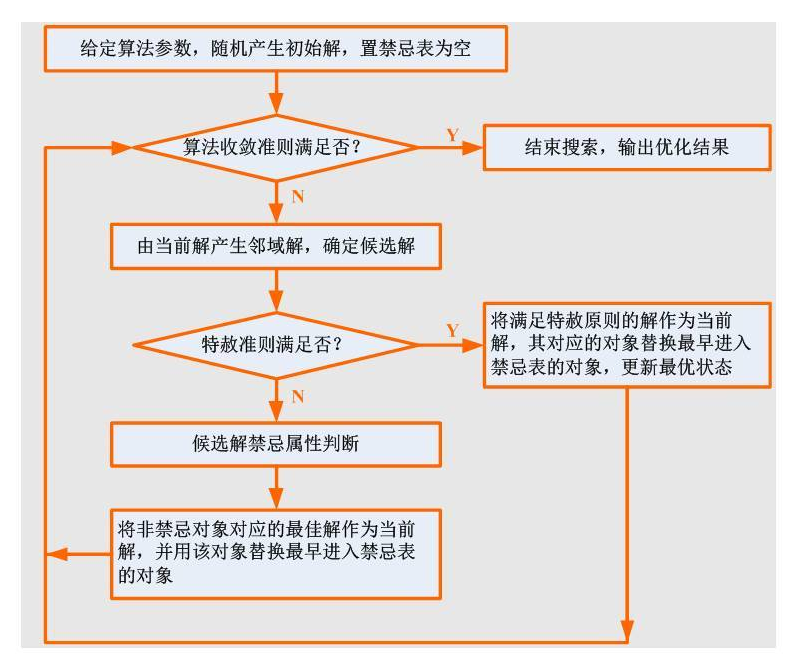
\includegraphics[width=0.8\textwidth]{12.png}
\end{figure}

\subsection{一种综合的禁忌算法}
下面我们总结一种相当一般的具有如上所述诸多特征的禁忌算法.在对指定问题的属性列表进行初始化以及识别后,此算法如下进行:
\begin{enumerate}
	\item 定义一个依赖于f的扩展目标函数$ f_{H^{(t)}} $,它也可能依赖于
	\begin{enumerate}
		\item 基于频率的惩罚或激励以提升多样化
		\item 基于频率的惩罚或激励以提升强化
	\end{enumerate}
	\item 确定$ \theta^{(t)} $的邻域,即$ N(\theta^{(t)}) $的元素.
	\item 按照由$ f_{H^{(t)}} $计算而得的改进量,求邻域的秩
	\item 选取秩最大的邻域.
	\item 此邻域是否在当前的禁忌列表中?不在的话,转第八步.
	\item 此邻域是否通过一个特设准则?通过则转第八步.
	\item 如果$ \theta^{(t)} $的所有邻域都考虑过了,且没有一个被所采用作为$ \theta^{(t+1)} $,则停止,否则选择秩次最高的邻域且转至第五步.
	\item 采用此解作为$ \theta^{(t+1)} $
	\item 通过建立基于当前移动的新禁忌或删除过期的禁忌来更新禁忌表.
	\item 符合一个停止准则吗?符合则停止,否则增加t并转至第一步.
\end{enumerate}

\section{模拟退火}
\textbf{模拟退火算法(Simulate Anneal Arithmetic,SAA)}是一种通用概率演算法,用来在一个大的搜寻空间内找寻命题的最优解。它是基于Monte-Carlo迭代求解策略的一种随机寻优算法。模拟退火算法是S.Kirkpatrick, C.D.Gelatt和M.P.Vecchi等人在1983年发明的,1985年,V.Černý也独立发明了此演算法。模拟退火算法是解决TSP问题的有效方法之一。

模拟退火算法来源于固体退火原理。 \textbf{物理退火: }将材料加热后再经特定速率冷却,目的是增大晶粒的体积,并且减少晶格中的缺陷。材料中的原子原来会停留在使内能有局部最小值的位置,加热使能量变大,原子会离开原来位置,而随机在其他位置中移动。退火冷却时速度较慢,使得原子有较多可能可以找到内能比原先更低的位置。 \textbf{模拟退火:} 其原理也和固体退火的原理近似。模拟退火算法从某一较高初温出发,伴随温度参数的不断下降,结合概率突跳特性在解空间中随机寻找目标函数的全局最优解,即在局部最优解能概率性地跳出并最终趋于全局最优。

爬山法是完完全全的贪心法,这种贪心是很鼠目寸光的,只把眼光放在局部最优解上,因此只能搜索到局部的最优值。模拟退火其实也是一种贪心算法,只不过与爬山法不同的是,模拟退火算法在搜索过程引入了随机因素。模拟退火算法以一定的概率来接受一个比当前解要差的解,因此有可能会跳出这个局部的最优解,达到全局的最优解。

\subsection{算法过程}
模拟退火算法是一个迭代算法,时刻$ t=0 $的初值为$ \theta^{(0)} $,温度为$ \tau_0 $.用t表示迭代,此算法在几个阶段内运行,且阶段标号为$ j=0,1,2,... $而每一个阶段均含有多步迭代.第j个阶段的长度为$ m_j $,每次迭代如下进行:
\begin{enumerate}
	\item 在$ \theta^{(t)} $的邻域$ N(\theta^{(t)}) $内,根据提案密度$ g^{(t)}(\cdot|\theta^{(t)}) $选取候选解$ \theta^{*}  $
	\item 随机决定是否采用$ \theta^* $作为下一个候选解或还是仍用当前解.特别地,以概率
	$$min(1,exp\left\lbrace \frac{f(\theta^{(t)} )-f(\theta^{*} )}{\tau_j}\right\rbrace )$$
	取$ \theta^{(t+1)}=\theta^*$,否则令$ \theta^{(t+1)} =\theta^{(t)}  $
	\item 重复第一二步$ m_j $次
	\item 增加j且更新$ \tau_j=\alpha(\tau_{j-1}),\;m_j=\beta(m_{j-1}) $,并转至第一步.
\end{enumerate}

如果根据总迭代次数的限制或事先给定的$ \tau_j $和$ m_j $,此算法不能停止,则人们可以用绝对或相对收敛准则来控制它.然而,停止准则多由最小温度来表示.算法停止后,所求得的最优候选解即是估计的最小值.

函数$ \alpha $应使温度慢慢递减至0.在每个温度$ m_j $中 的迭代次数应较大且关于j单增.理想的函数$ \beta $应使$ m_j $为p的指数,但在实际中为达到容许的计算速度进行某些折中是必要的.

尽管当一个候选解由于当前解使它总被采用,但注意当它不好时,它也有一定的概率被采用.在这种意义下,模拟退火算法是一种随机的下降算法.此随机性将使模拟退火算法有时能逃脱一个没有竞争力的局部极小值.

\subsubsection{邻域和提案密度}

选取领域结构的最关键一点就是允许在$ \Theta $中所有解都能沟通.为使$ \theta_i $与$ \theta_j $沟通,就必须找到一个有限解$ \theta_1,...,\theta_k $,使得$ \theta_1\in N(\theta_1),...,\theta_k\in N(\theta_k) $.

最常用的提案密度$ g^{(t)}(\cdot|\theta^{(t)}) $是离散均匀,此时的候选解为来自$ N(\theta^{(t)}) $的完全随机样本.
\subsubsection{冷却进度与收敛}
阶段长度和温度的序列称为\textbf{冷却进度}.理想的冷却进度应比较慢.模拟退火的极限行为来自第Ⅰ章介绍的马氏链理论.可以把模拟退火看成为生成一列齐次马氏链(每个温度一列)或一个非齐次马氏链(温度在转换间递减).尽管这种看法将导致定义极限行为方法的不同,但二者的结论均为:所得到的极限分布的支撑集仅在整体极小值集合上.

在实际中,人们尝试过许多冷却进度﹒回想一下在第j阶段的温度是
$ \tau_j=\alpha (\tau_{j-1}) $,第j阶段的迭代次数是$ m_j=\beta (m_{j-1}) $﹒一种常用的方法是对所有的j,
取$ m_j =1 $,且根据$ \alpha (\tau_{j-1})=\frac{\tau_{j-1}}{1+\alpha\tau_{j-1}}$,较慢地降低温度,其中$ \alpha $是一个小量.第二种
选择是取$ \alpha (\tau_{j-1})=a\tau_{j-1} $,其中a<1(一般地, a$ \geq $0.9).此时,人们可以在降低温度
时增加阶段长度.例如,考虑$ \beta(m_{j-1})= bm_{j-i}(b >1) $或$ \beta(m_{j-1})= b+m_{j-i}(b >1) $.\\

\begin{figure}[H]
	\centering
	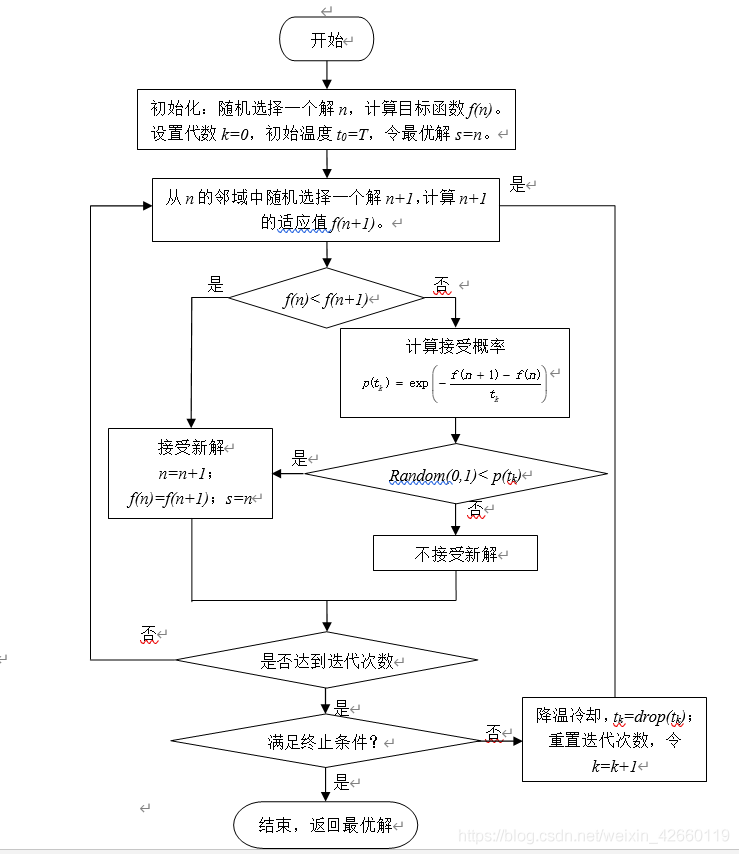
\includegraphics[width=0.8\textwidth]{23.png}
\end{figure}

\section{遗传算法}
\textbf{遗传算法(Genetic Algorithm)}遵循『适者生存』、『优胜劣汰』的原则,是一类借鉴生物界自然选择和自然遗传机制的随机化搜索算法。遗传算法模拟一个人工种群的进化过程,通过\textbf{选择(Selection)、交叉(Crossover)}以及\textbf{变异(Mutation)}等机制,\textbf{在每次迭代中都保留一组候选个体,重复此过程},种群经过若干代进化后,理想情况下其适应度达到\textbf{近似最优}的状态。自从遗传算法被提出以来,其得到了广泛的应用,特别是在函数优化、生产调度、模式识别、神经网络、自适应控制等领域,遗传算法发挥了很大的作用,提高了一些问题求解的效率。

\subsection{遗传算法组成}
\begin{tcolorbox}[colback=pink!10!white,colframe=pink!100!black]
\begin{itemize}
	\item 编码$ \rightarrow $创造染色体
	\item 个体$ \rightarrow $种群
	\item 适应度函数
	\item 遗传算子
	\item 选择
	\item 交叉
	\item 变异
\end{itemize}
\end{tcolorbox}

\textbf{运行参数}
\begin{itemize}
	\item 是否选择精英操作
	\item 种群大小
	\item 染色体长度
	\item 最大迭代次数
	\item 交叉概率
	\item 变异概率
\end{itemize}

\subsection{编码与解码}
实现遗传算法的第一步就是明确对求解问题的编码和解码方式。对于函数优化问题,一般有两种编码方式,各具优缺点:

\textbf{实数编码}:直接用实数表示基因,容易理解且不需要解码过程,但容易过早收敛,从而陷入局部最优.

\textbf{二进制编码}:稳定性高,种群多样性大,但需要的存储空间大,需要解码且难以理解对于求解函数最大值问题.

我选择的是二进制编码。


以我们的目标函数$  f(x)=x + 10\sin(5x)+7\cos(4x), x\in[0,9]  $为例。假如设定求解的精度为小数点后4位,可以将x的解空间划分为$  (9-0)\times(1e+4)=90000 $个等分。$ 2^{16}<90000<2^{17} $,需要17位二进制数来表示这些解。换句话说,一个解的编码就是一个17位的二进制串。一开始,这些二进制串是随机生成的。一个这样的二进制串代表一条染色体串,这里染色体串的长度为17。对于任何一条这样的染色体chromosome,如何将它复原(解码)到[0,9]这个区间中的数值呢?对于本问题,我们可以采用以下公式来解码:
\begin{equation}
x = 0 + decimal(chromosome)\times(9-0)/(2^{17}-1)
\end{equation}
decimal( ): 将二进制数转化为十进制数

一般化解码公式:
\begin{equation}
f(x), x\in[lower\_bound, upper\_bound]
\end{equation}
\begin{equation}
x = lower\_bound+decimal(chromosome)\times\frac{(upper\_bound-lower\_bound)}{(2^{chromosome\_size}-1)}
\end{equation}

lower\_bound: 函数定义域的下限

upper\_bound: 函数定义域的上限

chromosome\_size: 染色体的长度

通过上述公式,我们就可以成功地将二进制染色体串解码成[0,9]区间中的十进制实数解。


\subsection{个体与种群}
染色体表达了某种特征,这种特征的载体,称为『\textbf{个体}』。对于本次实验所要解决的一元函数最大值求解问题,个体可以用上一节构造的染色体表示,一个个体里有一条染色体。许多这样的个体组成了一个种群,其含义是一个一维点集(x轴上[0,9]的线段)。

\subsection{适应度函数}
遗传算法中,\textbf{一个个体(解)的好坏用适应度函数值来评价},在本问题中,$ f(x) $就是适应度函数。适应度函数值越大,解的质量越高。适应度函数是遗传算法进化的驱动力,也是进行自然选择的唯一标准,它的设计应结合求解问题本身的要求而定。

\subsection{遗传算子}
我们希望有这样一个种群,它所包含的个体所对应的函数值都很接近于f(x)在[0,9]上的最大值,但是这个种群一开始可能不那么优秀,因为个体的染色体串是随机生成的。如何让种群变得优秀呢?\textbf{不断的进化}。\textbf{每一次进化都尽可能保留种群中的优秀个体,淘汰掉不理想的个体,并且在优秀个体之间进行染色体交叉,有些个体还可能出现变异}。

种群的每一次进化,都会产生一个最优个体。种群所有世代的最优个体,可能就是函数$ f(x) $最大值对应的定义域中的点。如果种群无休止地进化,那总能找到最好的解。但实际上,我们的时间有限,通常在得到一个看上去不错的解时,便终止了进化。

对于给定的种群,如何赋予它进化的能力呢?

首先是\textbf{选择机制(selection)}.选择操作是从前代种群中选择\textbf{多对较优个体,选择用来产生子代的父代的一个过程.}一个最简单的方法就是以一个正比例于适宜度的概率选择一个父代,而完全随机地选择另一个父代.另一方法则是以正比例于适宜度地概率随机地选择每一个父代.

各个个体被选中的概率与其适应度函数值大小成正比轮盘赌选择方法具有随机性,在选择的过程中可能会丢掉较好的个体,所以可以使用精英机制,将前代最优个体直接选择.\\

由选定父代染色体得到子代染色体地方法就称\textbf{遗传算子(genetic operator)}

一个基本地遗传算子是\textbf{交叉互换(crossover)}.两个待交叉的不同的染色体(父母)根据交叉概率(cross\_rate)按某种方式交换其部分基因.采用单点交叉法,也可以使用其他交叉方法

另一个重要的遗传算子为\textbf{变异/突变(mutation)}.染色体按照变异概率(mutate\_rate)进行染色体的变异.采用单点变异法,也可以使用其他变异方法.

一般来说,\textbf{交叉概率(cross\_rate)比较大,变异概率(mutate\_rate)极低}。像求解函数最大值这类问题,我设置的交叉概率(cross\_rate)是0.6,变异概率(mutate\_rate)是0.01。

因为遗传算法相信2条优秀的父母染色体交叉更有可能产生优秀的后代,而变异的话产生优秀后代的可能性极低,不过也有存在可能一下就变异出非常优秀的后代。这也是符合自然界生物进化的特征的。

\subsection{遗传算法流程}
\begin{figure}[H]
	\centering
	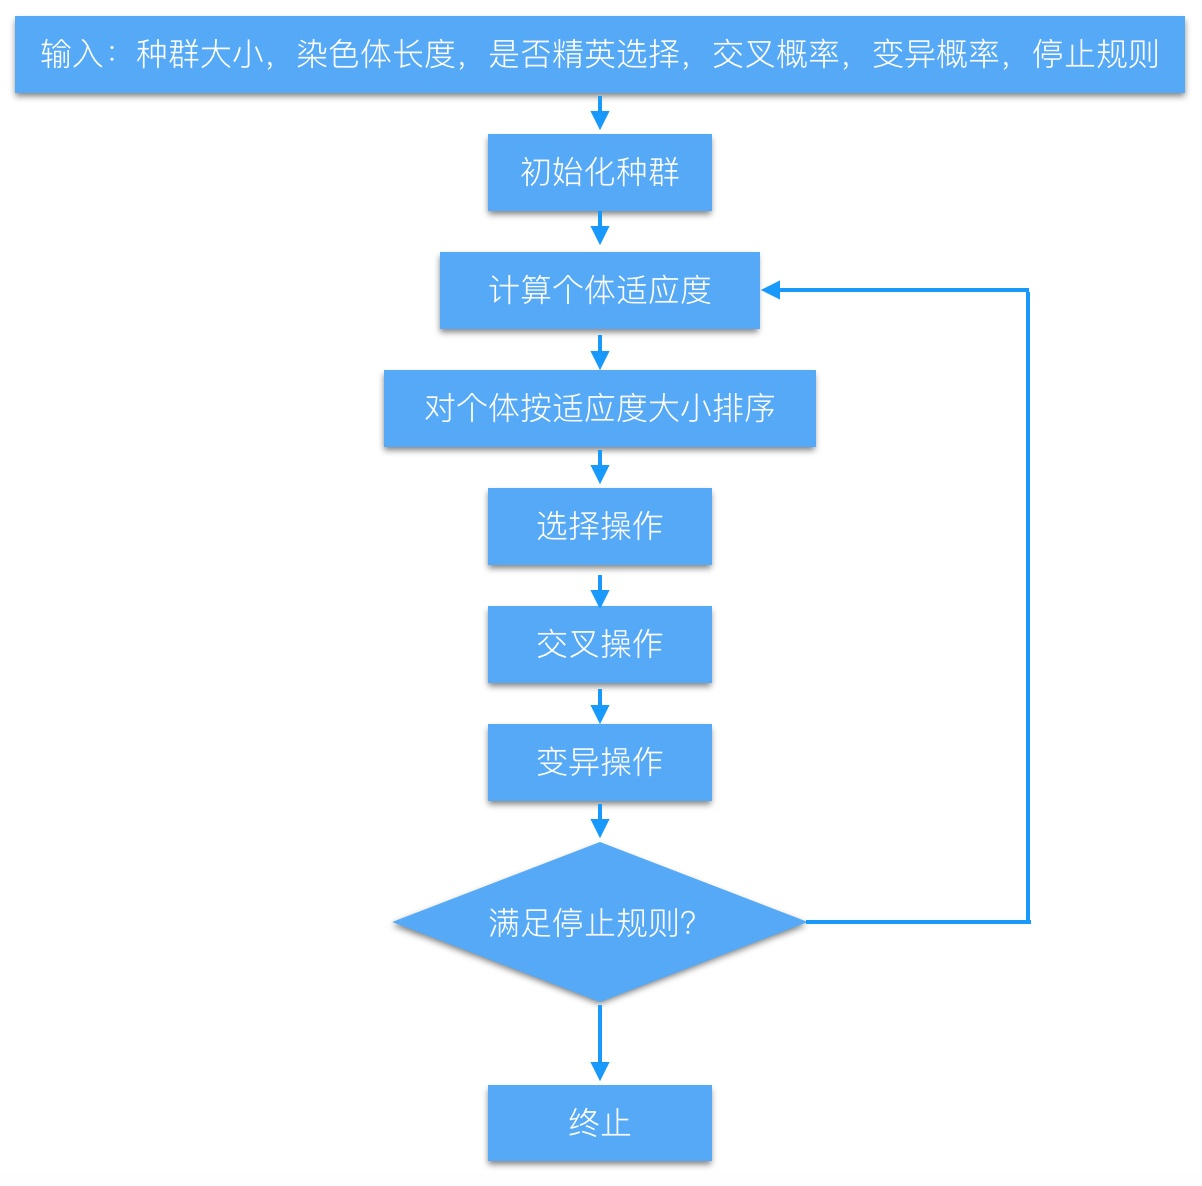
\includegraphics[width=0.7\textwidth]{15.jpg}
\end{figure}

\chapter{EM算法}
\section{简介}
\textbf{EM(Expectation-Maximum)算法}也称期望最大化算法,曾入选“数据挖掘十大算法”中,可见EM算法在机器学习、数据挖掘中的影响力。EM算法是最常见的\textbf{隐变量估计方法},在机器学习中有极为广泛的用途,例如常被用来学习高斯混合模型(Gaussian mixture model,简称GMM)的参数;隐式马尔科夫算法(HMM)、LDA主题模型的变分推断等等。本文就对EM算法的原理做一个详细的总结。

EM算法是一种迭代优化策略,由于它的计算方法中每一次迭代都分两步,其中一个为\textbf{期望步(E步)},另一个为\textbf{极大步(M步)},所以算法被称为EM算法(Expectation-Maximization Algorithm)。EM算法受到缺失思想影响,最初是为了解决数据缺失情况下的参数估计问题.\textbf{其基本思想是}:首先根据己经给出的观测数据,估计出模型参数的值;然后再依据上一步估计出的参数值估计缺失数据的值,再根据估计出的缺失数据加上之前己经观测到的数据重新再对参数值进行估计,然后反复迭代,直至最后收敛,迭代结束。
\section{预备知识}
想清晰的了解EM算法推导过程和其原理,我们需要知道两个基础知识:“极大似然估计”和“Jensen不等式”。

设f是定义域为实数的函数,如果对所有的实数x,f(x)的二阶导数都大于0,那么f是凸函数。如果f是凸函数,X是随机变量,那么
\begin{equation}
	\mathbb{E}[f(X)]\geq f(\mathbb{E}X)
\end{equation}
当且仅当X是常量时,该式取等号。其中,E(X)表示X的数学期望。

\section{EM算法详解}
\subsection{问题示例}
我们目前有100个男生和100个女生的身高,但是我们不知道这200个数据中哪个是男生的身高,哪个是女生的身高,即抽取得到的每个样本都不知道是从哪个分布中抽取的。这个时候,对于每个样本,就有两个未知量需要估计:

(1)这个身高数据是来自于男生数据集合还是来自于女生?

(2)男生、女生身高数据集的正态分布的参数分别是多少?
\begin{figure}[H]
	\centering
	
\includegraphics[width=0.7\textwidth]{16.jpg}
\end{figure}
那么,对于具体的身高问题使用EM算法求解步骤如图所示。
\begin{figure}[H]
	\centering
	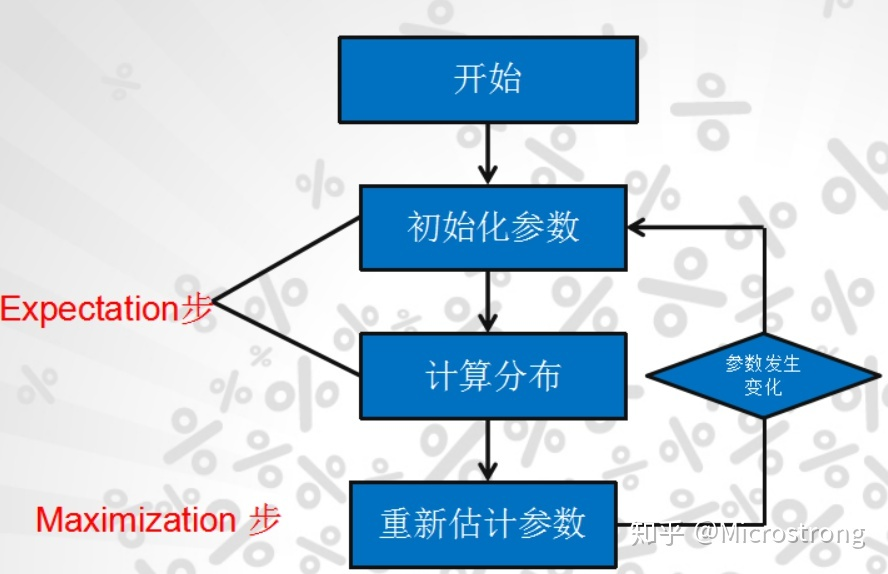
\includegraphics[width=0.7\textwidth]{17.jpg}
\end{figure}
\begin{enumerate}
	\item 初始化参数:先初始化男生身高的正态分布的参数:如均值=1.65,方差=0.15
	\item 计算每一个人更可能属于男生分布或者女生分布;
	\item 通过分为男生的n个人来重新估计男生身高分布的参数(最大似然估计),女生分布也按照相同的方式估计出来,更新分布。
	\item 这时候两个分布的概率也变了,然后重复步骤(1)至(3),直到参数不发生变化为止
\end{enumerate}

\subsection{EM算法推导流程}
\begin{tcolorbox}[colback=blue!7!white,colframe=blue!40]
	\textbf{arg}    是变元(即\textbf{自变量argument)}的英文缩写。
	
	arg min 就是使后面这个式子达到最小值时的变量的取值
	
	arg max 就是使后面这个式子达到最大值时的变量的取值
	
	例如 函数F(x,y):
	
	arg  min F(x,y)就是指当F(x,y)取得最小值时,变量x,y的取值
	
	arg  max F(x,y)就是指当F(x,y)取得最大值时,变量x,y的取值
\end{tcolorbox}
\begin{figure}[H]
	\centering
	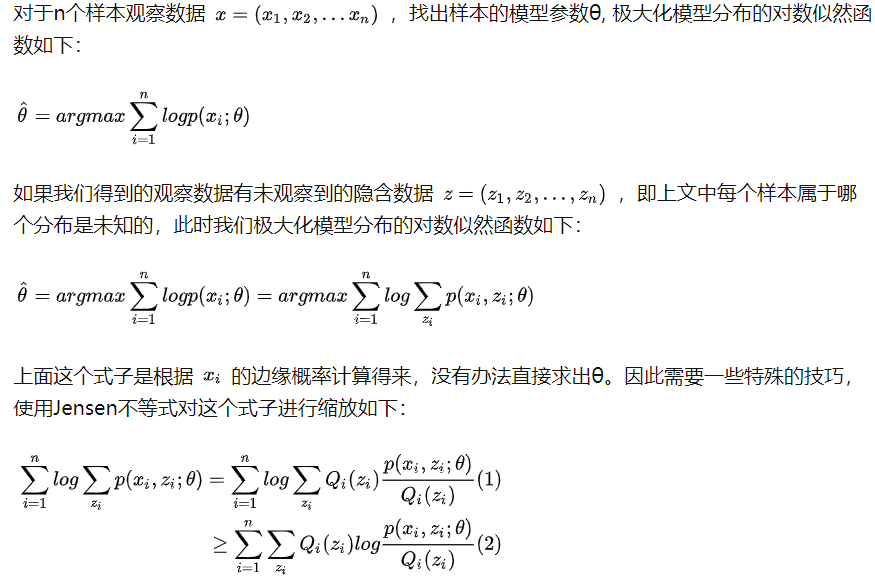
\includegraphics[width=\textwidth]{18.png}
\end{figure}
注意log函数为凹函数,故不等号反了过来.
\begin{figure}[H]
	\centering
	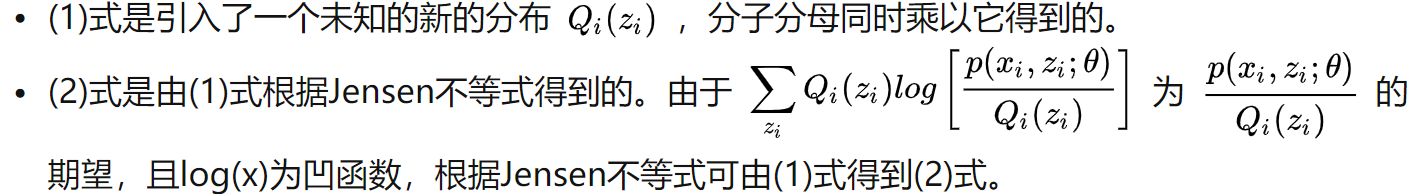
\includegraphics[width=\textwidth]{19.png}
\end{figure}
\begin{figure}[H]
	\centering
	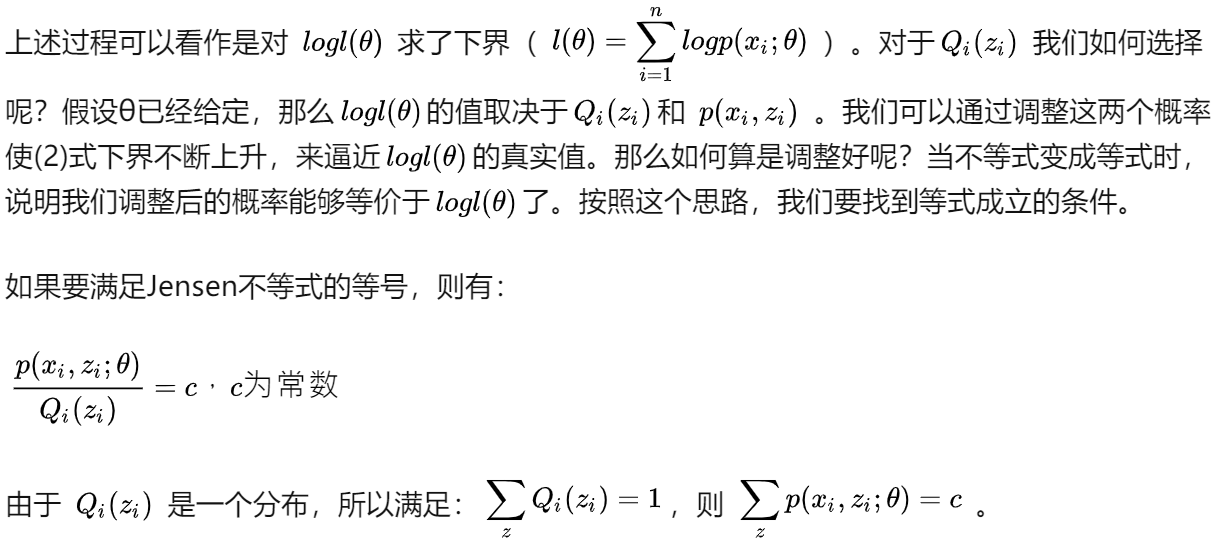
\includegraphics[width=\textwidth]{20.png}
\end{figure}
\begin{figure}[H]
	\centering
	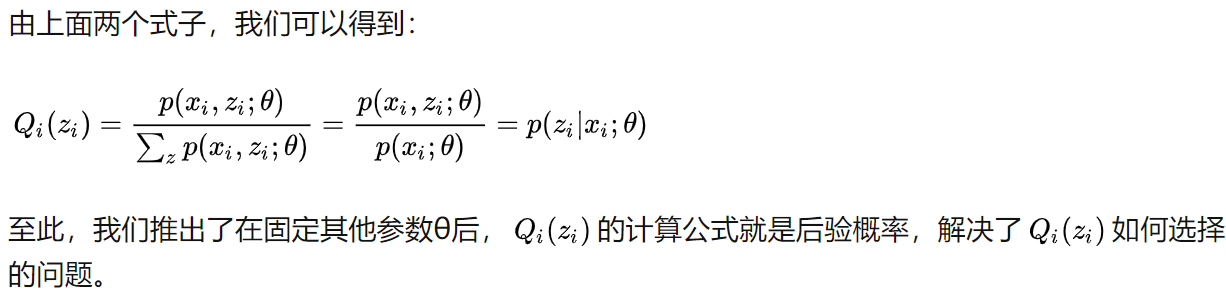
\includegraphics[width=\textwidth]{21.png}
\end{figure}
\begin{figure}[H]
	\centering
	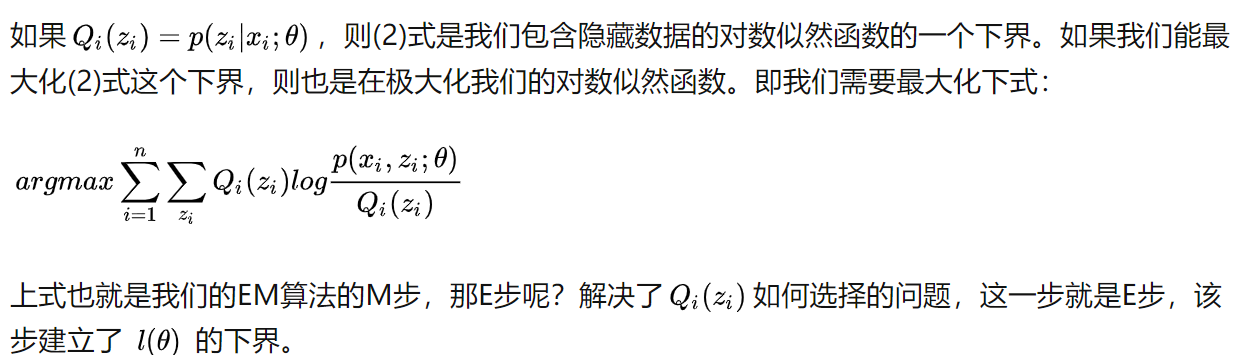
\includegraphics[width=\textwidth]{22.png}
\end{figure}
\section{EM算法流程}
\textbf{输入}: 观察到的数据$ x=(x_1,x_2,...,x_n) $,联合分布$ p(x,z;\theta) $,最大迭代次数$ J $.

\textbf{算法步骤}:
\begin{enumerate}
	\item 随机初始化模型参数$ \Theta $的初值$ \theta_0 $。
	\item j=1,2,...,J 开始EM算法迭代:
	
	\textbf{E步}:计算联合分布的条件概率期望
	\begin{equation}
	Q_i(z_i)=p(z_i|x_i,\theta_j)
	\end{equation}
	\begin{equation}
	l(\theta ,\theta_j)=\sum_{i=1}^{n}\sum_{z_i}Q_i(z_i)\log\frac{p(x_i,z_i;\theta)}{Q_i(z_i)}
	\end{equation}

	\textbf{M步}:极大化$ l(\theta ,\theta_j) $,得到$ \theta_{j+1} =\arg\max l(\theta ,\theta_j)$
	
	\item 如果$ \theta_{j+1} $已经收敛,则算法结束.否则继续进行E步和M步进行迭代.
\end{enumerate}

\textbf{输出}:模型参数$ \theta $
\begin{lstlisting}[language=r]
	
\end{lstlisting}
\begin{lstlisting}[language=r]
	
\end{lstlisting}
\begin{lstlisting}[language=r]
	
\end{lstlisting}
\begin{lstlisting}[language=r]
	
\end{lstlisting}



\end{document}